
\documentclass[twocolumn]{aastex62}
%\documentclass[defaultstyle,11pt]{thesis}
%\documentclass[]{report}
%\documentclass[]{article}
%\usepackage{aastex_hack}
%\usepackage{deluxetable}
%\documentclass[preprint]{aastex}
%\documentclass{aa}

\newcommand{\titlerunning}[1]{\shorttitle{#1}}
\newcommand{\authorrunning}[1]{\shortauthors{#1}}

\newcommand*\inst[1]{\unskip\hbox{\@textsuperscript{\normalfont$#1$}}}

%\newcount\aa@nbinstitutes
%
%\newcounter{aa@institutecnt}

\newcommand*\institute[1]{
  \begingroup
    \let\and\relax
    \renewcommand*\inst[1]{}%
    \renewcommand*\thanks[1]{}%
    \renewcommand*\email[1]{}%
    %\let\@@protect\protect
    %\let\protect\@unexpandable@protect
    %\global\aa@nbinstitutes \z@
    %\expandafter\aa@cntinstitutes\aa@institute\and\aa@nil\and
    %\restore@protect
  \endgroup
  \newcommand{\institutions}{#1}
}%

\let\oldarcsec\arcsec
\renewcommand\arcsec{\oldarcsec\xspace}%

%\renewcommand{\abstract}[1]{
%\begin{abstract}
%    #1
%\end{abstract}
%}

%\renewcommand\ion[2]{#1$\;${%
%\ifx\@currsize\normalsize\small \else
%\ifx\@currsize\small\footnotesize \else
%\ifx\@currsize\footnotesize\scriptsize \else
%\ifx\@currsize\scriptsize\tiny \else
%\ifx\@currsize\large\normalsize \else
%\ifx\@currsize\Large\large
%\fi\fi\fi\fi\fi\fi
%\rmfamily\@Roman{#2}}\relax}% 
%
%\renewcommand{ion}[2]{#1}{#2}

\renewcommand{\ion}[2]{\textup{#1\,\textsc{\lowercase{#2}}}}

%\newcommand{\uchii}{\ensuremath{\mathrm{\ion{UCH}{2}}}\xspace}
%\newcommand{\UCHII}{\ensuremath{\mathrm{\ion{UCH}{2}}}\xspace}
%\newcommand{\hchii}{\ensuremath{\mathrm{\ion{HCH}{2}}}\xspace}
%\newcommand{\HCHII}{\ensuremath{\mathrm{\ion{HCH}{2}}}\xspace}
%\newcommand{\hii}  {\ensuremath{\mathrm{\ion{H}{2}}}\xspace}

%\input{aamacros.tex}

\pdfminorversion=4


%%%%%%%%%%%%%%%%%%%%%%%%%%%%%%%%%%%%%%%%%%%%%%%%%%%%%%%%%%%%%%%%
%%%%%%%%%%%  see documentation for information about  %%%%%%%%%%
%%%%%%%%%%%  the options (11pt, defaultstyle, etc.)   %%%%%%%%%%
%%%%%%%  http://www.colorado.edu/its/docs/latex/thesis/  %%%%%%%
%%%%%%%%%%%%%%%%%%%%%%%%%%%%%%%%%%%%%%%%%%%%%%%%%%%%%%%%%%%%%%%%
%		\documentclass[typewriterstyle]{thesis}
% 		\documentclass[modernstyle]{thesis}
% 		\documentclass[modernstyle,11pt]{thesis}
%	 	\documentclass[modernstyle,12pt]{thesis}

%%%%%%%%%%%%%%%%%%%%%%%%%%%%%%%%%%%%%%%%%%%%%%%%%%%%%%%%%%%%%%%%
%%%%%%%%%%%    load any packages which are needed    %%%%%%%%%%%
%%%%%%%%%%%%%%%%%%%%%%%%%%%%%%%%%%%%%%%%%%%%%%%%%%%%%%%%%%%%%%%%
\usepackage{latexsym}		% to get LASY symbols
\usepackage{graphicx}		% to insert PostScript figures
%\usepackage{deluxetable}
\usepackage{rotating}		% for sideways tables/figures
\usepackage{natbib}  % Requires natbib.sty, available from http://ads.harvard.edu/pubs/bibtex/astronat/
\usepackage{savesym}
%\usepackage{pdflscape}
\usepackage{amssymb}
\usepackage{amsmath}
\usepackage{morefloats}
%\savesymbol{singlespace}
\savesymbol{doublespace}
%\usepackage{wrapfig}
%\usepackage{setspace}
\usepackage{xspace}
\usepackage{color}
%\usepackage{multicol}
\usepackage{mdframed}
\usepackage{url}
\usepackage{subfigure}
%\usepackage{emulateapj}
%\usepackage{lscape}
\usepackage{grffile}
\usepackage{import}
\usepackage[utf8]{inputenc}
%\usepackage{longtable}
\usepackage{booktabs}
%\usepackage[yyyymmdd,hhmmss]{datetime}
\usepackage{fancyhdr}
%\usepackage[colorlinks=true,citecolor=blue,linkcolor=cyan]{hyperref}

\usepackage[hang,flushmargin]{footmisc}
\usepackage{ifpdf}


%\usepackage{standalone}
%\standalonetrue






\newcommand{\paa}{Pa\ensuremath{\alpha}}
\newcommand{\brg}{Br\ensuremath{\gamma}}
\newcommand{\msun}{\ensuremath{M_{\odot}}\xspace}			%  Msun
\newcommand{\mdot}{\ensuremath{\dot{M}}\xspace}
\newcommand{\lsun}{\ensuremath{L_{\odot}}\xspace}			%  Lsun
\newcommand{\rsun}{\ensuremath{R_{\odot}}\xspace}			%  Rsun
\newcommand{\lbol}{\ensuremath{L_{\mathrm{bol}}\xspace}}	%  Lbol
\newcommand{\ks}{K\ensuremath{_{\mathrm{s}}}}		%  Ks
\newcommand{\hh}{\ensuremath{\textrm{H}_{2}}\xspace}			%  H2
\newcommand{\dens}{\ensuremath{n(\hh) [\percc]}\xspace}
\newcommand{\formaldehyde}{\ensuremath{\textrm{H}_2\textrm{CO}}\xspace}
\newcommand{\formamide}{\ensuremath{\textrm{NH}_2\textrm{CHO}}\xspace}
\newcommand{\formaldehydeIso}{\ensuremath{\textrm{H}_2~^{13}\textrm{CO}}\xspace}
\newcommand{\methanol}{\ensuremath{\textrm{CH}_3\textrm{OH}}\xspace}
\newcommand{\ortho}{\ensuremath{\textrm{o-H}_2\textrm{CO}}\xspace}
\newcommand{\para}{\ensuremath{\textrm{p-H}_2\textrm{CO}}\xspace}
\newcommand{\oneone}{\ensuremath{1_{1,0}-1_{1,1}}\xspace}
\newcommand{\twotwo}{\ensuremath{2_{1,1}-2_{1,2}}\xspace}
\newcommand{\threethree}{\ensuremath{3_{1,2}-3_{1,3}}\xspace}
\newcommand{\threeohthree}{\ensuremath{3_{0,3}-2_{0,2}}\xspace}
\newcommand{\threetwotwo}{\ensuremath{3_{2,2}-2_{2,1}}\xspace}
\newcommand{\threetwoone}{\ensuremath{3_{2,1}-2_{2,0}}\xspace}
\newcommand{\fourtwotwo}{\ensuremath{4_{2,2}-3_{1,2}}\xspace} % CH3OH 218.4 GHz
\newcommand{\methylcyanide}{\ensuremath{\textrm{CH}_{3}\textrm{CN}}\xspace}
\newcommand{\ketene}{\ensuremath{\textrm{H}_{2}\textrm{CCO}}\xspace}
\newcommand{\ethylcyanide}{\ensuremath{\textrm{CH}_3\textrm{CH}_2\textrm{CN}}\xspace}
\newcommand{\cyanoacetylene}{\ensuremath{\textrm{HC}_{3}\textrm{N}}\xspace}
\newcommand{\methylformate}{\ensuremath{\textrm{CH}_{3}\textrm{OCHO}}\xspace}
\newcommand{\dimethylether}{\ensuremath{\textrm{CH}_{3}\textrm{OCH}_{3}}\xspace}
\newcommand{\gaucheethanol}{\ensuremath{\textrm{g-CH}_3\textrm{CH}_2\textrm{OH}}\xspace}
\newcommand{\acetone}{\ensuremath{\left[\textrm{CH}_{3}\right]_2\textrm{CO}}\xspace}
\newcommand{\methyleneamidogen}{\ensuremath{\textrm{H}_{2}\textrm{CN}}\xspace}
\newcommand{\Rone}{\ensuremath{\para~S_{\nu}(\threetwoone) / S_{\nu}(\threeohthree)}\xspace}
\newcommand{\Rtwo}{\ensuremath{\para~S_{\nu}(\threetwotwo) / S_{\nu}(\threetwoone)}\xspace}
\newcommand{\JKaKc}{\ensuremath{J_{K_a K_c}}}
\newcommand{\water}{H$_{2}$O\xspace}		%  H2O
\newcommand{\feii}{\ion{Fe}{ii}\xspace}		%  FeII

\newcommand{\uchii}{\ion{UCH}{ii}\xspace}
\newcommand{\UCHII}{\ion{UCH}{ii}\xspace}
\newcommand{\hchii}{\ion{HCH}{ii}\xspace}
\newcommand{\HCHII}{\ion{HCH}{ii}\xspace}
\newcommand{\hii}{\ion{H}{ii}\xspace}

\newcommand{\hi}{H~{\sc i}\xspace}
\newcommand{\Hii}{\hii}
\newcommand{\HII}{\hii}
\newcommand{\Xform}{\ensuremath{X_{\formaldehyde}}}
\newcommand{\kms}{\textrm{km~s}\ensuremath{^{-1}}\xspace}	%  km s-1
\newcommand{\nsample}{456\xspace}
\newcommand{\CFR}{5\xspace} % nMPC / 0.25 / 2 (6 for W51 once, 8 for W51 twice) REFEDIT: With f_observed=0.3, becomes 3/2./0.3 = 5
\newcommand{\permyr}{\ensuremath{\mathrm{Myr}^{-1}}\xspace}
\newcommand{\pers}{\ensuremath{\mathrm{s}^{-1}}\xspace}
\newcommand{\perspc}{\ensuremath{\mathrm{pc}^{-2}}\xspace}
\newcommand{\tsuplim}{0.5\xspace} % upper limit on starless timescale
\newcommand{\ncandidates}{18\xspace}
\newcommand{\mindist}{8.7\xspace}
\newcommand{\rcluster}{2.5\xspace}
\newcommand{\ncomplete}{13\xspace}
\newcommand{\middistcut}{13.0\xspace}
\newcommand{\nMPC}{3\xspace} % only count W51 once.  W51, W49, G010
\newcommand{\obsfrac}{30}
\newcommand{\nMPCtot}{10\xspace} % = nmpc / obsfrac
\newcommand{\nMPCtoterr}{6\xspace} % = sqrt(nmpc) / obsfrac
\newcommand{\plaw}{2.1\xspace}
\newcommand{\plawerr}{0.3\xspace}
\newcommand{\mmin}{\ensuremath{10^4~\msun}\xspace}
%\newcommand{\perkmspc}{\textrm{per~km~s}\ensuremath{^{-1}}\textrm{pc}\ensuremath{^{-1}}\xspace}	%  km s-1 pc-1
\newcommand{\kmspc}{\textrm{km~s}\ensuremath{^{-1}}\textrm{pc}\ensuremath{^{-1}}\xspace}	%  km s-1 pc-1
\newcommand{\sqcm}{cm$^{2}$\xspace}		%  cm^2
\newcommand{\percc}{\ensuremath{\textrm{cm}^{-3}}\xspace}
\newcommand{\perpc}{\ensuremath{\textrm{pc}^{-1}}\xspace}
\newcommand{\persc}{\ensuremath{\textrm{cm}^{-2}}\xspace}
\newcommand{\persr}{\ensuremath{\textrm{sr}^{-1}}\xspace}
\newcommand{\peryr}{\ensuremath{\textrm{yr}^{-1}}\xspace}
\newcommand{\perkmspc}{\textrm{km~s}\ensuremath{^{-1}}\textrm{pc}\ensuremath{^{-1}}\xspace}	%  km s-1 pc-1
\newcommand{\perkms}{\textrm{per~km~s}\ensuremath{^{-1}}\xspace}	%  km s-1 
\newcommand{\um}{\ensuremath{\mu \textrm{m}}\xspace}    % micron
\newcommand{\microjy}{\ensuremath{\mu\textrm{Jy}}\xspace}    % micron
\newcommand{\microJy}{\ensuremath{\mu\textrm{Jy}}\xspace}    % micron
\newcommand{\mum}{\um}
\newcommand{\htwo}{\ensuremath{\textrm{H}_2}}
\newcommand{\Htwo}{\ensuremath{\textrm{H}_2}}
\newcommand{\HtwoO}{\ensuremath{\textrm{H}_2\textrm{O}}}
\newcommand{\htwoo}{\ensuremath{\textrm{H}_2\textrm{O}}}
\newcommand{\ha}{\ensuremath{\textrm{H}\alpha}}
\newcommand{\hb}{\ensuremath{\textrm{H}\beta}}
\newcommand{\so}{SO~\ensuremath{5_6-4_5}\xspace}
\newcommand{\SO}{SO~\ensuremath{1_2-1_1}\xspace}
\newcommand{\ammonia}{NH\ensuremath{_3}\xspace}
\newcommand{\twelveco}{\ensuremath{^{12}\textrm{CO}}\xspace}
\newcommand{\thirteenco}{\ensuremath{^{13}\textrm{CO}}\xspace}
\newcommand{\ceighteeno}{\ensuremath{\textrm{C}^{18}\textrm{O}}\xspace}
\def\ee#1{\ensuremath{\times10^{#1}}}
\newcommand{\degrees}{\ensuremath{^{\circ}}}
% can't have \degree because I'm getting a degree...
\newcommand{\lowirac}{800}
\newcommand{\highirac}{8000}
\newcommand{\lowmips}{600}
\newcommand{\highmips}{5000}
\newcommand{\perbeam}{\ensuremath{\textrm{beam}^{-1}}\xspace}
\newcommand{\ds}{\ensuremath{\textrm{d}s}}
\newcommand{\dnu}{\ensuremath{\textrm{d}\nu}}
\newcommand{\dv}{\ensuremath{\textrm{d}v}}
\def\secref#1{Section \ref{#1}}
\def\eqref#1{Equation \ref{#1}}
\def\facility#1{#1}
%\newcommand{\arcmin}{'}

\newcommand{\necluster}{Sh~2-233IR~NE}
\newcommand{\swcluster}{Sh~2-233IR~SW}
\newcommand{\region}{IRAS 05358}

\newcommand{\nwfive}{40}
\newcommand{\nouter}{15}

\newcommand{\vone}{{\rm v}1.0\xspace}
\newcommand{\vtwo}{{\rm v}2.0\xspace}
\newcommand\mjysr{\ensuremath{{\rm MJy~sr}^{-1}}}
\newcommand\jybm{\ensuremath{{\rm Jy~bm}^{-1}}}
\newcommand\nbolocat{8552\xspace}
\newcommand\nbolocatnew{548\xspace}
\newcommand\nbolocatnonew{8004\xspace} % = nbolocat-nbolocatnew
%\renewcommand\arcdeg{\mbox{$^\circ$}\xspace} 
%\renewcommand\arcmin{\mbox{$^\prime$}\xspace} 
%\renewcommand\arcsec{\mbox{$^{\prime\prime}$}\xspace} 

\newcommand{\todo}[1]{\textcolor{red}{#1}}
\newcommand{\okinfinal}[1]{{#1}}
%% only needed if not aastex
%\newcommand{\keywords}[1]{}
%\newcommand{\email}[1]{}
%\newcommand{\affil}[1]{}


%aastex hack
%\newcommand\arcdeg{\mbox{$^\circ$}}%
%\newcommand\arcmin{\mbox{$^\prime$}\xspace}%
%\newcommand\arcsec{\mbox{$^{\prime\prime}$}\xspace}%

%\newcommand\epsscale[1]{\gdef\eps@scaling{#1}}
%
%\newcommand\plotone[1]{%
% \typeout{Plotone included the file #1}
% \centering
% \leavevmode
% \includegraphics[width={\eps@scaling\columnwidth}]{#1}%
%}%
%\newcommand\plottwo[2]{{%
% \typeout{Plottwo included the files #1 #2}
% \centering
% \leavevmode
% \columnwidth=.45\columnwidth
% \includegraphics[width={\eps@scaling\columnwidth}]{#1}%
% \hfil
% \includegraphics[width={\eps@scaling\columnwidth}]{#2}%
%}}%


%\newcommand\farcm{\mbox{$.\mkern-4mu^\prime$}}%
%\let\farcm\farcm
%\newcommand\farcs{\mbox{$.\!\!^{\prime\prime}$}}%
%\let\farcs\farcs
%\newcommand\fp{\mbox{$.\!\!^{\scriptscriptstyle\mathrm p}$}}%
%\newcommand\micron{\mbox{$\mu$m}}%
%\def\farcm{%
% \mbox{.\kern -0.7ex\raisebox{.9ex}{\scriptsize$\prime$}}%
%}%
%\def\farcs{%
% \mbox{%
%  \kern  0.13ex.%
%  \kern -0.95ex\raisebox{.9ex}{\scriptsize$\prime\prime$}%
%  \kern -0.1ex%
% }%
%}%

\def\Figure#1#2#3#4#5{
\begin{figure*}[!htp]
\includegraphics[scale=#4,width=#5]{#1}
\caption{#2}
\label{#3}
\end{figure*}
}

\def\FigureOneCol#1#2#3#4#5{
\begin{figure}[!htp]
\includegraphics[scale=#4,width=#5]{#1}
\caption{#2}
\label{#3}
\end{figure}
}


\def\WrapFigure#1#2#3#4#5#6{
\begin{wrapfigure}{#6}{0.5\textwidth}
\includegraphics[scale=#4,width=#5]{#1}
\caption{#2}
\label{#3}
\end{wrapfigure}
}

% % #1 - filename
% % #2 - caption
% % #3 - label
% % #4 - epsscale
% % #5 - R or L?
% \def\WrapFigure#1#2#3#4#5#6{
% \begin{wrapfigure}[#6]{#5}{0.45\textwidth}
% %  \centercaption
% %  \vspace{-14pt}
%   \epsscale{#4}
%   \includegraphics[scale=#4]{#1}
%   \caption{#2}
%   \label{#3}
% \end{wrapfigure}
% }

\def\RotFigure#1#2#3#4#5{
\begin{sidewaysfigure*}[!htp]
\includegraphics[scale=#4,width=#5]{#1}
\caption{#2}
\label{#3}
\end{sidewaysfigure*}
}

\def\FigureSVG#1#2#3#4{
\begin{figure*}[!htp]
    \def\svgwidth{#4}
    \input{#1}
    \caption{#2}
    \label{#3}
\end{figure*}
}

% originally intended to be included in a two-column paper
% this is in includegraphics: ,width=3in
% but, not for thesis
\def\OneColFigure#1#2#3#4#5{
\begin{figure}[!htpb]
\epsscale{#4}
\includegraphics[scale=#4,angle=#5]{#1}
\caption{#2}
\label{#3}
\end{figure}
}

\def\SubFigure#1#2#3#4#5{
\begin{figure*}[!htp]
\addtocounter{figure}{-1}
\epsscale{#4}
\includegraphics[angle=#5]{#1}
\caption{#2}
\label{#3}
\end{figure*}
}


\def\FigureTwo#1#2#3#4#5#6{
\begin{figure*}[!htp]
\subfigure[]{ \includegraphics[scale=#5,width=#6]{#1} }
\subfigure[]{ \includegraphics[scale=#5,width=#6]{#2} }
\caption{#3}
\label{#4}
\end{figure*}
}

\def\FigureTwoAA#1#2#3#4#5#6{
\begin{figure*}[!htp]
\subfigure[]{ \includegraphics[scale=#5,width=#6]{#1} }
\subfigure[]{ \includegraphics[scale=#5,width=#6]{#2} }
\caption{#3}
\label{#4}
\end{figure*}
}

\newenvironment{rotatepage}
{}{}


\def\RotFigureTwoAA#1#2#3#4#5#6{
\begin{rotatepage}
\begin{sidewaysfigure*}[!htp]
\subfigure[]{ \includegraphics[scale=#5,width=#6]{#1} }
\\
\subfigure[]{ \includegraphics[scale=#5,width=#6]{#2} }
\caption{#3}
\label{#4}
\end{sidewaysfigure*}
\end{rotatepage}
}

\def\RotFigureThree#1#2#3#4#5#6#7{
\begin{rotatepage}
\begin{sidewaysfigure*}[!htp]
\subfigure[]{ \includegraphics[scale=#6,width=#7]{#1} }
\\
\subfigure[]{ \includegraphics[scale=#6,width=#7]{#2} }
\\
\subfigure[]{ \includegraphics[scale=#6,width=#7]{#3} }
\caption{#4}
\label{#5}
\end{sidewaysfigure*}
\end{rotatepage}
\clearpage
}

\def\FigureThree#1#2#3#4#5#6#7{
\begin{figure*}[!htp]
\subfigure[]{ \includegraphics[scale=#6,width=#7]{#1} }
\subfigure[]{ \includegraphics[scale=#6,width=#7]{#2} }
\subfigure[]{ \includegraphics[scale=#6,width=#7]{#3} }
\caption{#4}
\label{#5}
\end{figure*}
}



\def\SubFigureTwo#1#2#3#4#5{
\begin{figure*}[!htp]
\addtocounter{figure}{-1}
\epsscale{#5}
\plottwo{#1}{#2}
\caption{#3}
\label{#4}
\end{figure*}
}

\def\FigureFour#1#2#3#4#5#6#7#8{
\begin{figure*}[!htp]
\subfigure[]{ \includegraphics[scale=#7,width=#8]{#1} }
\subfigure[]{ \includegraphics[scale=#7,width=#8]{#2} }
\subfigure[]{ \includegraphics[scale=#7,width=#8]{#3} }
\subfigure[]{ \includegraphics[scale=#7,width=#8]{#4} }
\caption{#5}
\label{#6}
\end{figure*}
}

\def\FigureFourVertical#1#2#3#4#5#6#7#8{
\begin{figure*}[!htp]
\subfigure[]{ \includegraphics[scale=#7,width=#8]{#1} }
\vspace{0.001mm} \\
\subfigure[]{ \includegraphics[scale=#7,width=#8]{#2} }
\vspace{0.001mm} \\
\subfigure[]{ \includegraphics[scale=#7,width=#8]{#3} }
\vspace{0.001mm} \\
\subfigure[]{ \includegraphics[scale=#7,width=#8]{#4} }
\vspace{0.001mm}
\caption{#5}
\label{#6}
\end{figure*}
}

\def\FigureFourPDF#1#2#3#4#5#6{
\begin{figure*}[!htp]
\subfigure[]{ \includegraphics[width=3in,type=pdf,ext=.pdf,read=.pdf]{#1} }
\subfigure[]{ \includegraphics[width=3in,type=pdf,ext=.pdf,read=.pdf]{#2} }
\subfigure[]{ \includegraphics[width=3in,type=pdf,ext=.pdf,read=.pdf]{#3} }
\subfigure[]{ \includegraphics[width=3in,type=pdf,ext=.pdf,read=.pdf]{#4} }
\caption{#5}
\label{#6}
\end{figure*}
}

\def\FigureThreePDF#1#2#3#4#5{
\begin{figure*}[!htp]
\subfigure[]{ \includegraphics[width=3in,type=pdf,ext=.pdf,read=.pdf]{#1} }
\subfigure[]{ \includegraphics[width=3in,type=pdf,ext=.pdf,read=.pdf]{#2} }
\subfigure[]{ \includegraphics[width=3in,type=pdf,ext=.pdf,read=.pdf]{#3} }
\caption{#4}
\label{#5}
\end{figure*}
}

\def\Table#1#2#3#4#5{
%\renewcommand{\thefootnote}{\alph{footnote}}
\begin{table}
\caption{#2}
\label{#3}
    \begin{tabular}{#1}
        \hline\hline
        #4
        \hline
        #5
        \hline
    \end{tabular}
\end{table}
%\renewcommand{\thefootnote}{\arabic{footnote}}
}


%\def\Table#1#2#3#4#5#6{
%%\renewcommand{\thefootnote}{\alph{footnote}}
%\begin{deluxetable}{#1}
%\tablewidth{0pt}
%\tabletypesize{\footnotesize}
%\tablecaption{#2}
%\tablehead{#3}
%\startdata
%\label{#4}
%#5
%\enddata
%\bigskip
%#6
%\end{deluxetable}
%%\renewcommand{\thefootnote}{\arabic{footnote}}
%}

%\def\tablenotetext#1#2{
%\footnotetext[#1]{#2}
%}

% \def\LongTable#1#2#3#4#5#6#7#8{
% % required to get tablenotemark to work: http://www2.astro.psu.edu/users/stark/research/psuthesis/longtable.html
% \renewcommand{\thefootnote}{\alph{footnote}}
% \begin{longtable}{#1}
% \caption[#2]{#2}
% \label{#4} \\
% 
%  \\
% \hline 
% #3 \\
% \hline
% \endfirsthead
% 
% \hline
% #3 \\
% \hline
% \endhead
% 
% \hline
% \multicolumn{#8}{r}{{Continued on next page}} \\
% \hline
% \endfoot
% 
% \hline 
% \endlastfoot
% #7 \\
% 
% #5
% \hline
% #6 \\
% 
% \end{longtable}
% \renewcommand{\thefootnote}{\arabic{footnote}}
% }

\def\TallFigureTwo#1#2#3#4#5#6{
\begin{figure*}[htp]
\epsscale{#5}
\subfigure[]{ \includegraphics[width=#6]{#1} }
\subfigure[]{ \includegraphics[width=#6]{#2} }
\caption{#3}
\label{#4}
\end{figure*}
}

		% file containing author's macro definitions
%%% This file is generated by the Makefile.
\newcommand{\githash}{008e348}\newcommand{\gitdate}{2018-10-19\xspace}\newcommand{\gitauthor}{Adam Ginsburg (keflavich)\xspace}

\newcommand{\sourcei}{SrcI\xspace}
\newcommand{\sourcen}{SrcN\xspace}
\newcommand{\sourcex}{SrcX\xspace}
\newcommand{\bam}[1]{\textcolor{green!65!black}{\textbf{[BAM: #1]}}}
\newcommand{\ag}[1]{\textcolor{red!65!black}{\textbf{[AG: #1]}}}
\begin{document}
\newcommand{\nraojansky}{\affiliation{\it{Jansky fellow of the National Radio Astronomy Observatory, 1003 Lopezville Rd, Socorro, NM 87801 USA }}}
\newcommand{\nrao}{\affiliation{\it{National Radio Astronomy Observatory, 1003 Lopezville Rd, Socorro, NM 87801 USA }}}
\newcommand{\nraocv}{\affiliation{\it{National Radio Astronomy Observatory, Charlottesville, VA 22903 USA }}}
\newcommand{\cfa}{\affiliation{\it{Harvard-Smithsonian Center for Astrophysics, Cambridge, MA 02138 USA }}}
\newcommand{\hubble}{\altaffiliation{B.A.M. is a Hubble Fellow of the National Radio Astronomy\\ Observatory.}}


\newcommand{\radboud}{\affiliation{\it{Department of Astrophysics/IMAPP, Radboud University Nijmegen, PO Box 9010, 6500 GL Nijmegen, the Netherlands}}}
\newcommand{\allegro}{\affiliation{\it{ALLEGRO/Leiden Observatory, Leiden University, PO Box 9513, 2300 RA Leiden, the Netherlands}}}
\newcommand{\casa}{\affiliation{\it{CASA, University of Colorado, 389-UCB, Boulder, CO 80309}} }

\newcommand{\berkeley}{\affiliation{\it{Radio Astronomy Laboratory, University of California, Berkeley, CA 94720}} }

\author[0000-0001-6431-9633]{Adam Ginsburg}
\nraojansky
%\eso

%\author{
%Adam Ginsburg{\nrao},
%\begin{flushleft}
%\institutions
%\end{flushleft}
%        }
%
%\institute{
%    {\nrao}{\it{National Radio Astronomy Observatory, Socorro, NM 87801 USA\\
%                      \email{aginsbur@nrao.edu} 
%                      }} \\
%    }
%
\correspondingauthor{Adam Ginsburg}
\email{aginsbur@nrao.edu; adam.g.ginsburg@gmail.com}

\author{Brett McGuire}
\hubble
\nraocv
\cfa

\author{Richard Plambeck}
\berkeley

\author{John Bally}
\casa

\author{Ciriaco Goddi}
\allegro
\radboud


\author{Melvyn Wright}
\berkeley


\title{Orion \sourcei's disk is salty}
\begin{abstract}
    We report the detection of NaCl and KCl and their $^{37}$Cl and $^{41}$K
    isotopologues toward the disk around Orion \sourcei.
    This is the first detection of these molecules in the interstellar
    medium not associated with the ejecta of evolved stars.  It is also
    the first ever detection of the vibrationally excited states of these
    lines in the ISM, up to v=8.
    These lines are likely to be unique tracers of a rare process, either
    the birth of high-mass stars or the aftermath of a stellar collision.
\end{abstract}

\section{Introduction}
Molecules consisting of alkali metals and halogens have only rarely been
detected in space  \citep[e.g., see the review
by][]{XXX} \bam{This reference in the list points to another 2018 paper at the moment, not the review, which is 'in press.'}.   Because of their rarity, their use as a diagnostic
tool to measure metallicity and local physical conditions has been limited.
However, some of these molecules, such as KCl and NaCl, have a rich spectrum
with dozens of lines arising in a single observing band with modern
instrumentation, so they have great potential when they are detected.

They \bam{What is they? KCl and NaCl or all metal-halides?  Depending on the answer, I would start this sentence as either 'KCl and NaCl ...' or 'Metal-halides...'} have so far been observed toward evolved stars including the carbon star IRC
+10216 \citep{Cernicharo1987a}, oxygen-rich evolved stars IK Tauri and VY Canis
Majoris \citep{Milam2007a}, the post-AGB star envelope CRL 2688
\citep{Highberger2003a}, and the AGB star wind around OH 231+4.2
\citep{Sanchez-Contreras2018a}.  In these sources, they exist only in a limited
range of radii from the central star.  The limited environments in which these molecules have been
detected suggests that they only exist in the gas phase for a brief period when
being ejected from dying stars before being incorporated into dust grains.

% \bam{Did we check w/ Holger here to see where he thought
% the v=1 for NaCl was seen?  I still can't find a paper w/ it.  It's also
% probably not correct to cite my paper here - I haven't (yet) compiled
% vibrational information...} \ag{I haven't e-mailed him; you want to do that?
% I was just citing your paper since the information came from your brain...
% we ought to cite you somewhere, if not here}

The environments around forming stars, however, are also known to harbor molecules that are often rapidly depleted from the gas-phase after ejection.  Disks around forming high-mass stars have been resolved only a handful of times.  The disk around Orion Source I (\sourcei) has frequently been observed
\citep{Hirota2014a,Plambeck2016a,Ginsburg2018b}, but most molecular species
detected trace either an outflow (e.g., SiO) or some combination of the outflow
and the disk (e.g., \water).  In HH80/81, a $\sim4$ \msun disk around a
$\sim10-20$ \msun star, several lines of SO$_2$ are associated with the disk
\citep{Girart2017a}.  Beyond these two sources, only disordered structures or
disk-envelope blends have been observed.
% \bam{In HH80/81, or do you mean beyond
% this pair only disordered blends have been observed period, anywhere?}
% \ag{AFAIK, except for the HH80/81 and \sourcei disks, all disks around massive
% stars are ambiguous / not strictly disks.}

In \citet{Ginsburg2018b}, we used lines of \water and one or
more unknown species to measure the rotation curve of the disk around \sourcei.
We have now identified these unknown lines as transitions of NaCl and KCl.

\section{Observations and Analysis}

The pure-rotational spectra of KCl and its rare isotopologues was reported by \citet{Caris2004a} up to 930~GHz.  Most isotopologues were measured up to the seventh excited vibrational state.  \citet{Caris2004a} also refine predictions for NaCl based on prior laboratory work (again to 930~GHz) reported by \citet{Caris2002a}.  The results of these works were then subsequently used by \citet{Barton2014a} to generate high-temperature line lists, primarily for use in exoplanet atmospheres, and includes over 10$^5$ transitions for each molecular species and isotopologue with levels up to $E_U\sim5\ee{4}$ K. The primary result for the purposes of this work is the prediction of frequencies in vibrational states higher than those measured in the laboratory. To our knowledge, prior to this work, no astronomical detections of vibrationally excited transitions of either of these species, or their isotopologues, have been reported.

\bam{I can't follow your bibtex commands all that well, so I'm not sure where to put the new reference.  It is Caris et al. 2002 Z Naturforsch. 57a, 663.}

The observations presented here are described in \citet{Ginsburg2018b} as part
of ALMA project 2016.1.00165.S.  We use the robust 0.5 weighted spectral cubes
from all three bands (B3 3 mm, B6 1 mm, B7 0.85 mm) for our spectroscopic analysis.

Appendix D of that paper describes the spectral extraction method,
which we summarize here.  We used the U232.511 line (which we identify here as
NaCl v=1 J=18-17) to create a velocity centroid map.  For each spectrum in the
line data cube with
a measured velocity in this line, we shift the spectrum to 0 \kms, 
creating a cube in which all spectra have the same centroid velocity but retain
their original spectral profiles.  We then then averaged those
spectra over the region with significant emission in the bright NaCl line.  The
averaging area is approximately the extent of the continuum disk, 0.03 square
arcseconds, or about 4, 20, and 40  beam areas, resulting
in an improvement in the signal-to-noise of about $2\times$, $4\times$, and $6\times$
respectively in Band 3, 6, and 7.
This stacked spectrum, shown in Figures \ref{fig:spectrab3}-\ref{fig:spectrab7},
is the average spectrum across the disk identified in \citet{Ginsburg2018b}:
it traces material just above and below the optically thick continuum disk
(Figure \ref{fig:spatial}), and for the lines discussed here, includes no
emission associated with the outflow.  Note that because it averages spectra
at the disk ends, where the line is broadened by the line-of-sight motion,
and spectra toward the disk center, where they are narrow, the line widths
in the stacked spectra are somewhat broader than the intrinsic line width.


We have clearly identified the carrier of the majority of unidentified lines in
the \citet{Ginsburg2018b} spectra (only 2-3 lines are unidentified in the B6/B7
spectra, though there are several in B3 we have not identified).  The
detected lines have amplitudes in the range 0.5-3 mJy \perbeam, corresponding
to brightness temperatures 5-20 K.  In the appendix of \citet{Ginsburg2018b}, we reported that ``there is no
consistent pattern to the detected lines and no individual species can explain
more than a few of the observed lines.''  This statement was incorrect, as
there are obvious carriers for the majority of the unidentified lines that we
had simply overlooked: NaCl, KCl, and their isotopologues.

Figures \ref{fig:spectrab3}-\ref{fig:spectrab7} shows the spectra with lines labeled.  We have labeled all of the
detections and marginal detections of salt lines.  We also labeled the most
prominent outflow (e.g., SiO and H$_2$O) lines.
%We additionally labeled
%\emph{some} of the lines that were not detected because of severe confusion

\begin{figure*}[!htp]
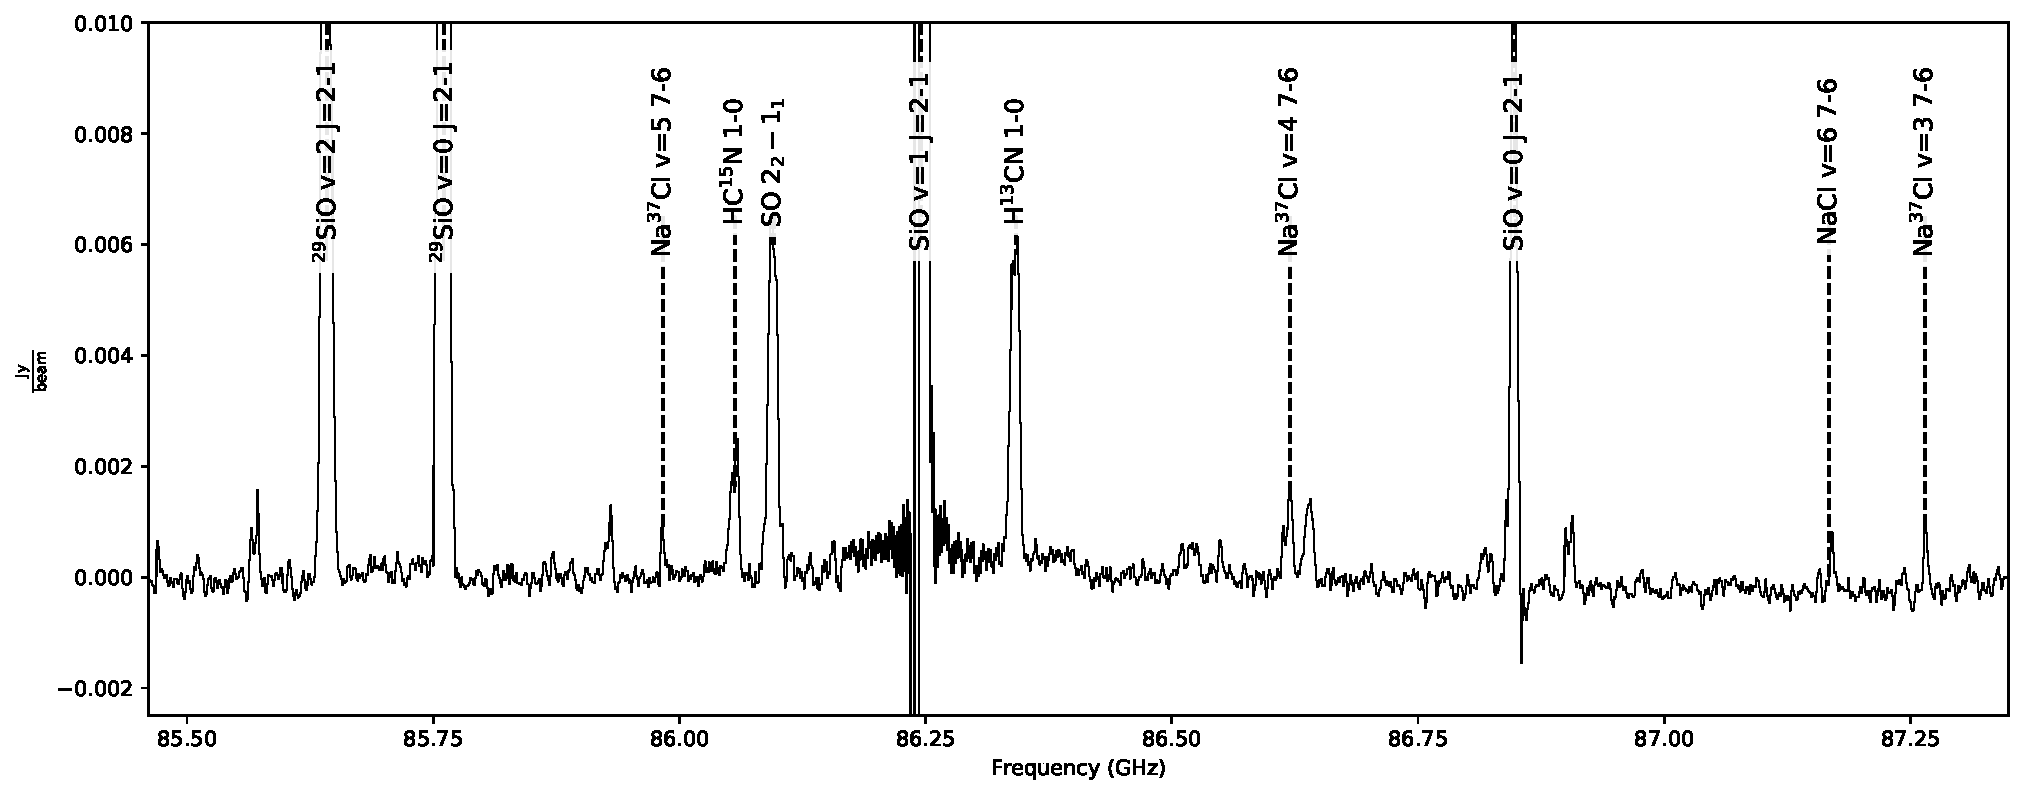
\includegraphics[scale=1,width=5.5in]{figures/lines_labeled_OrionSourceI_B3_spw0_robust0.5.pdf}
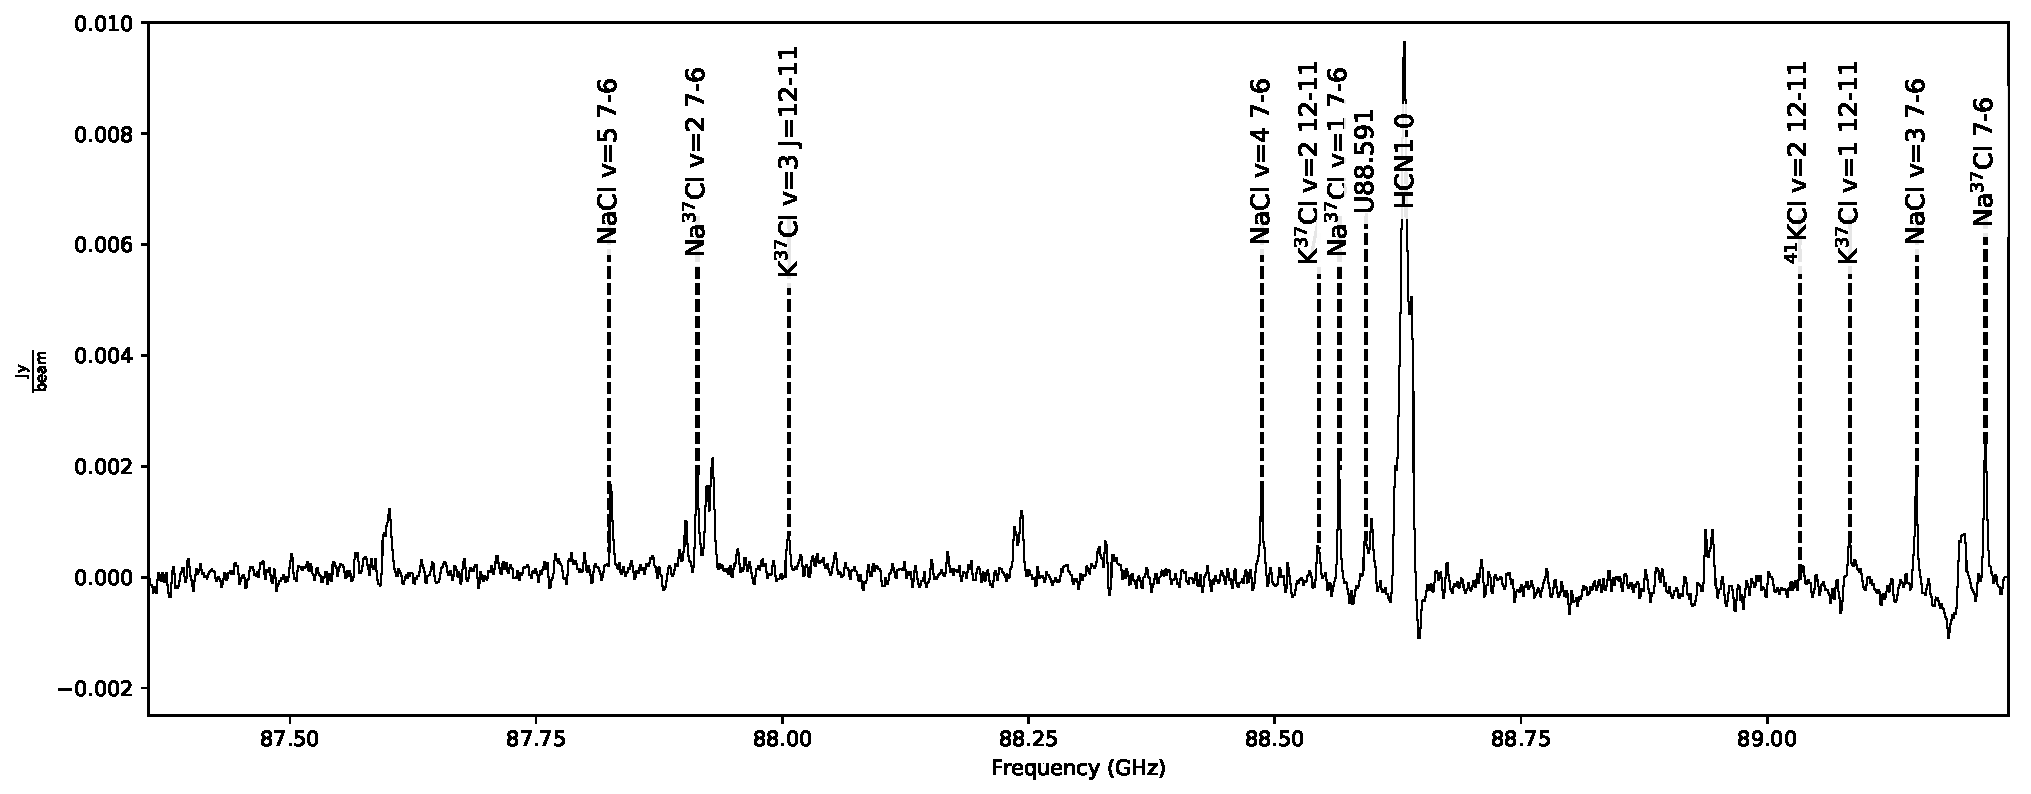
\includegraphics[scale=1,width=5.5in]{figures/lines_labeled_OrionSourceI_B3_spw1_robust0.5.pdf}
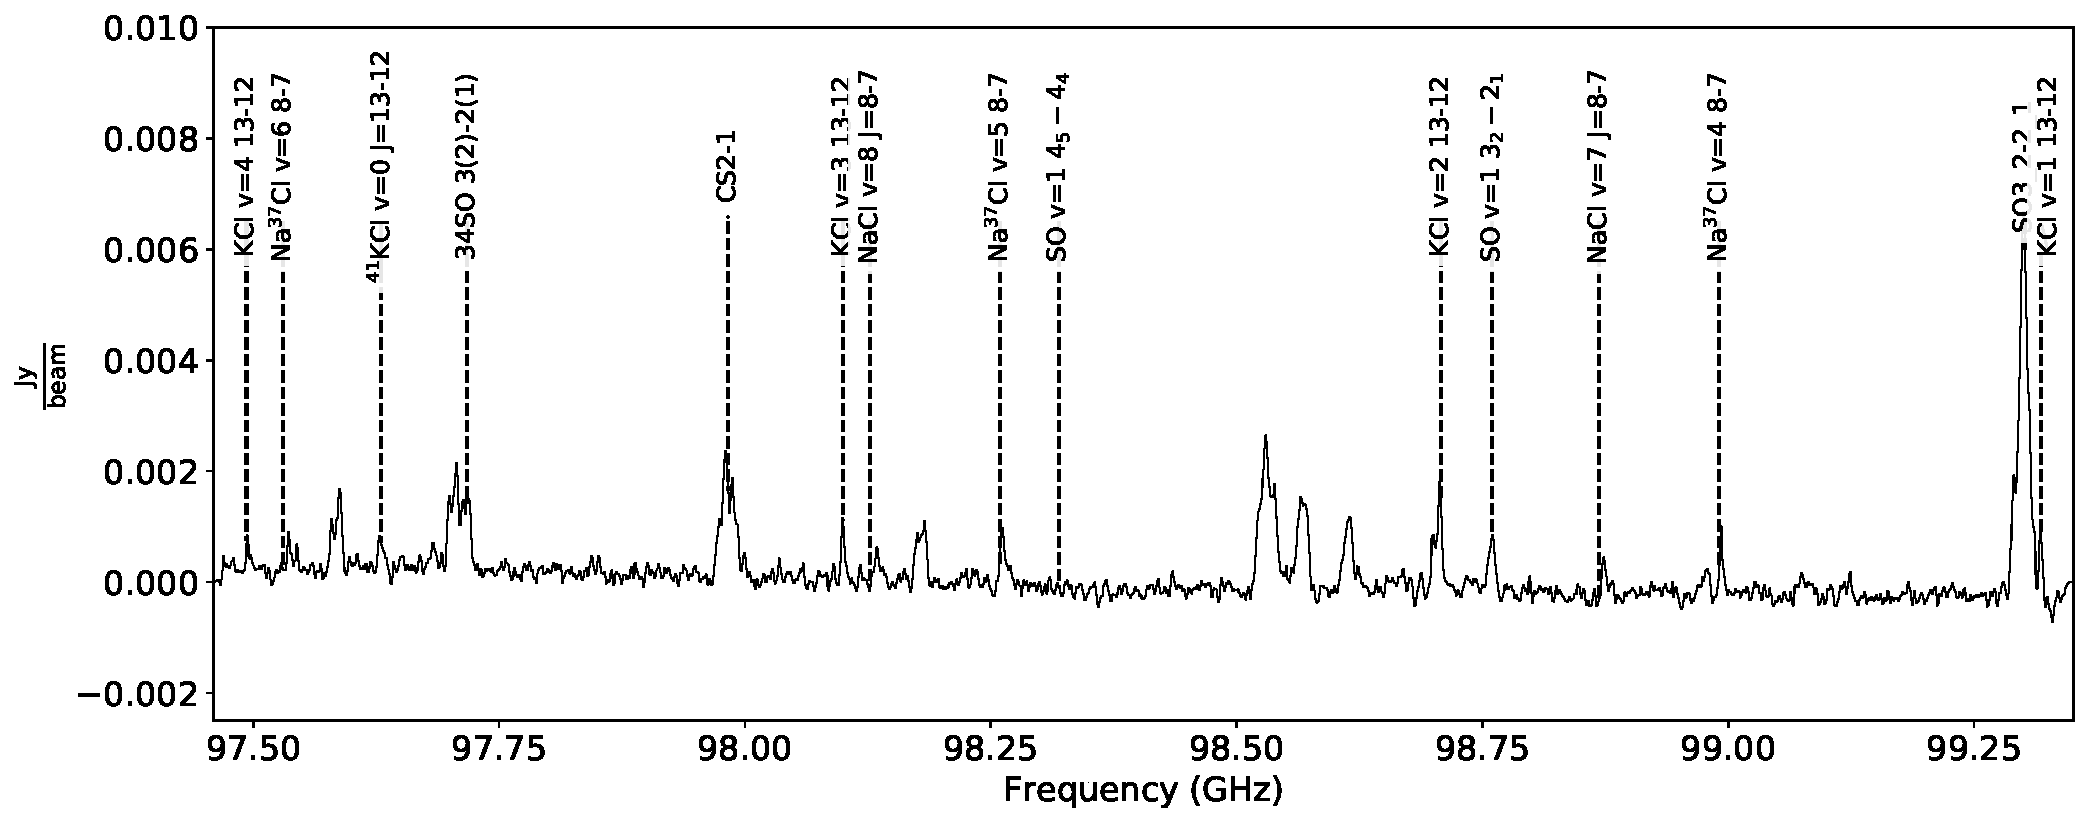
\includegraphics[scale=1,width=5.5in]{figures/lines_labeled_OrionSourceI_B3_spw2_robust0.5.pdf}
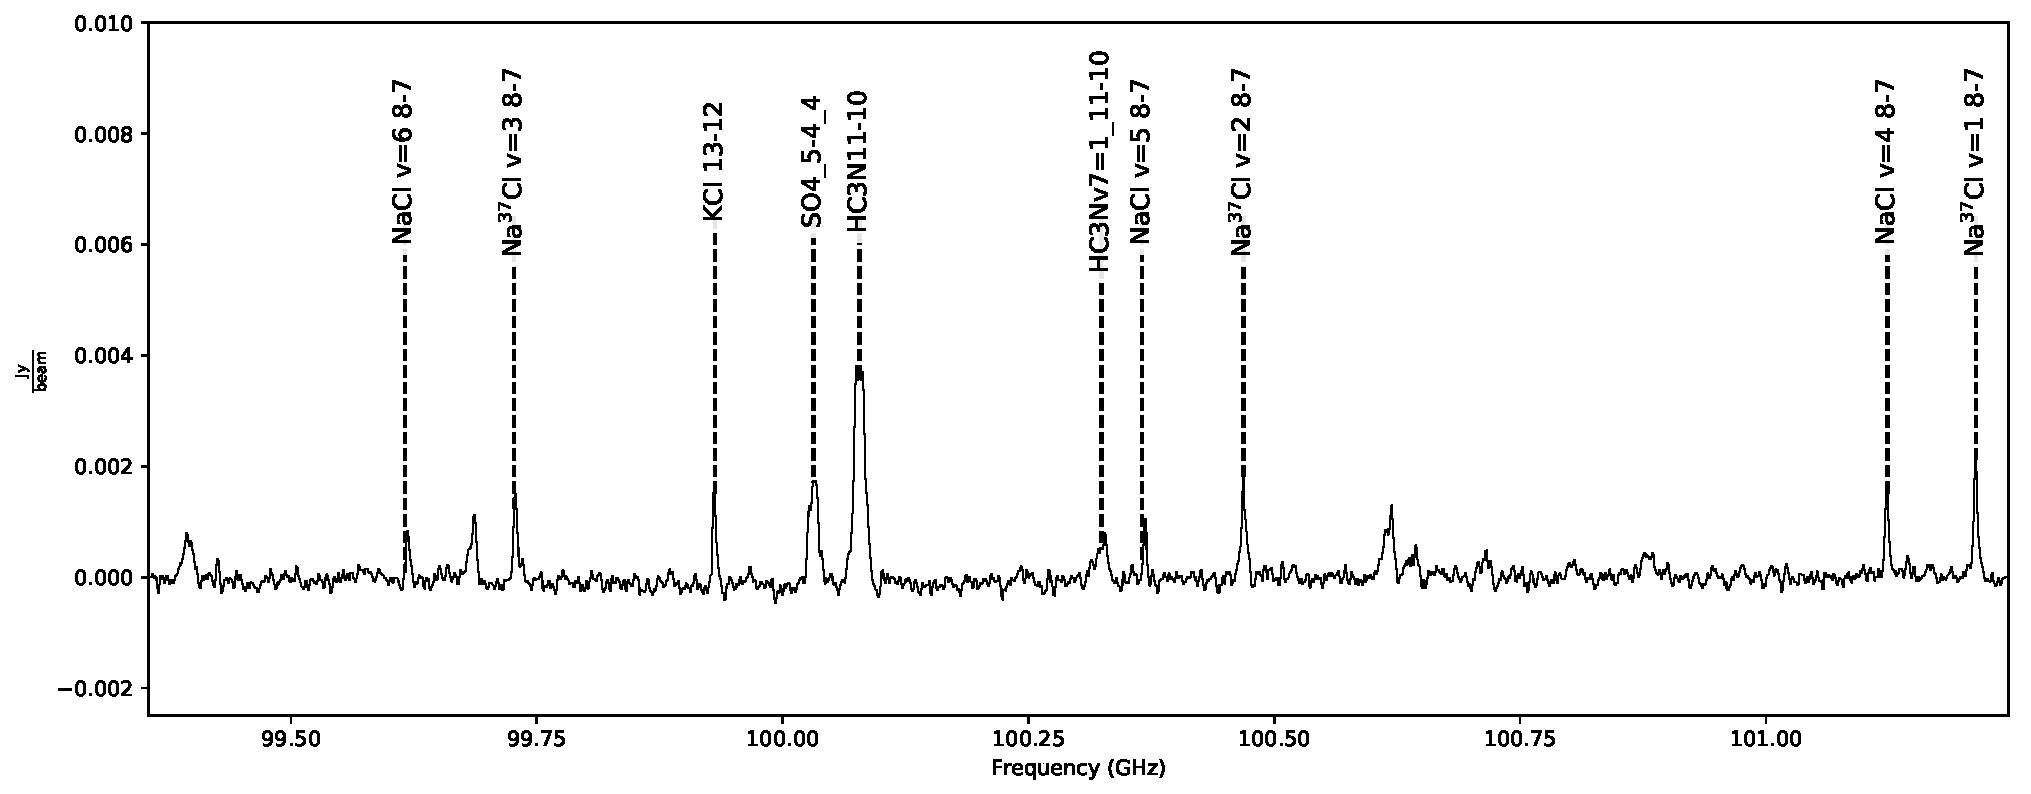
\includegraphics[scale=1,width=5.5in]{figures/lines_labeled_OrionSourceI_B3_spw3_robust0.5.pdf}
\caption{Stacked spectra  B3}
\label{fig:spectrab3}
\end{figure*}
\begin{figure*}[!htp]
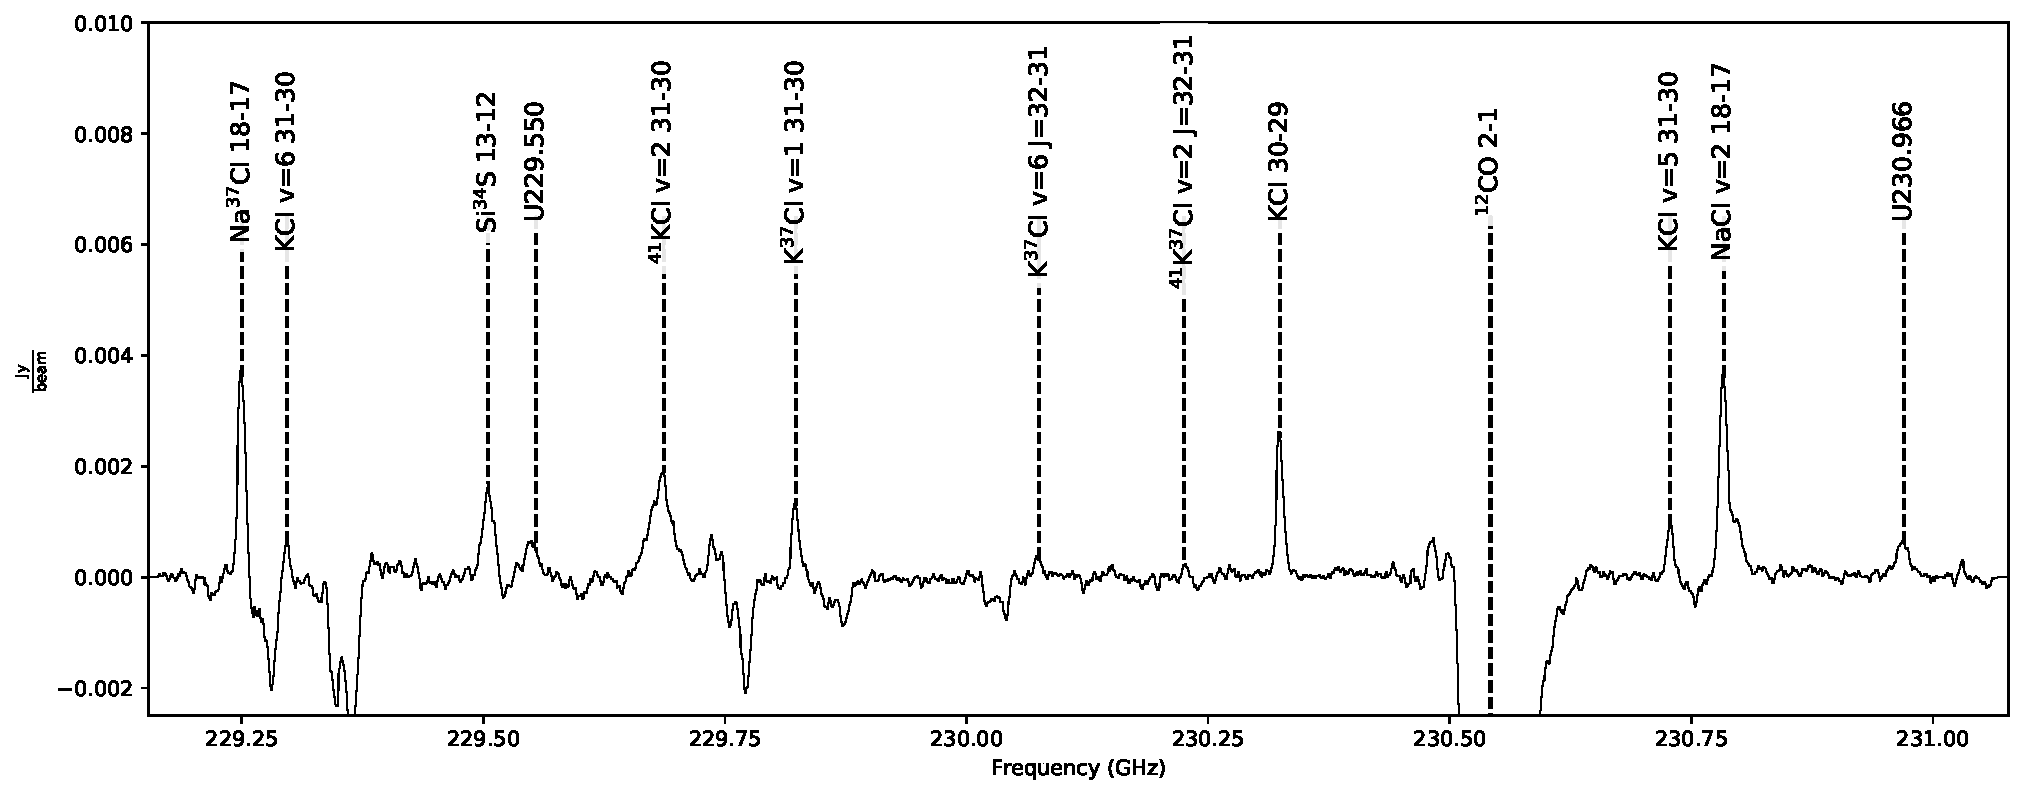
\includegraphics[scale=1,width=5.5in]{figures/lines_labeled_OrionSourceI_B6_spw0_robust0.5.pdf}
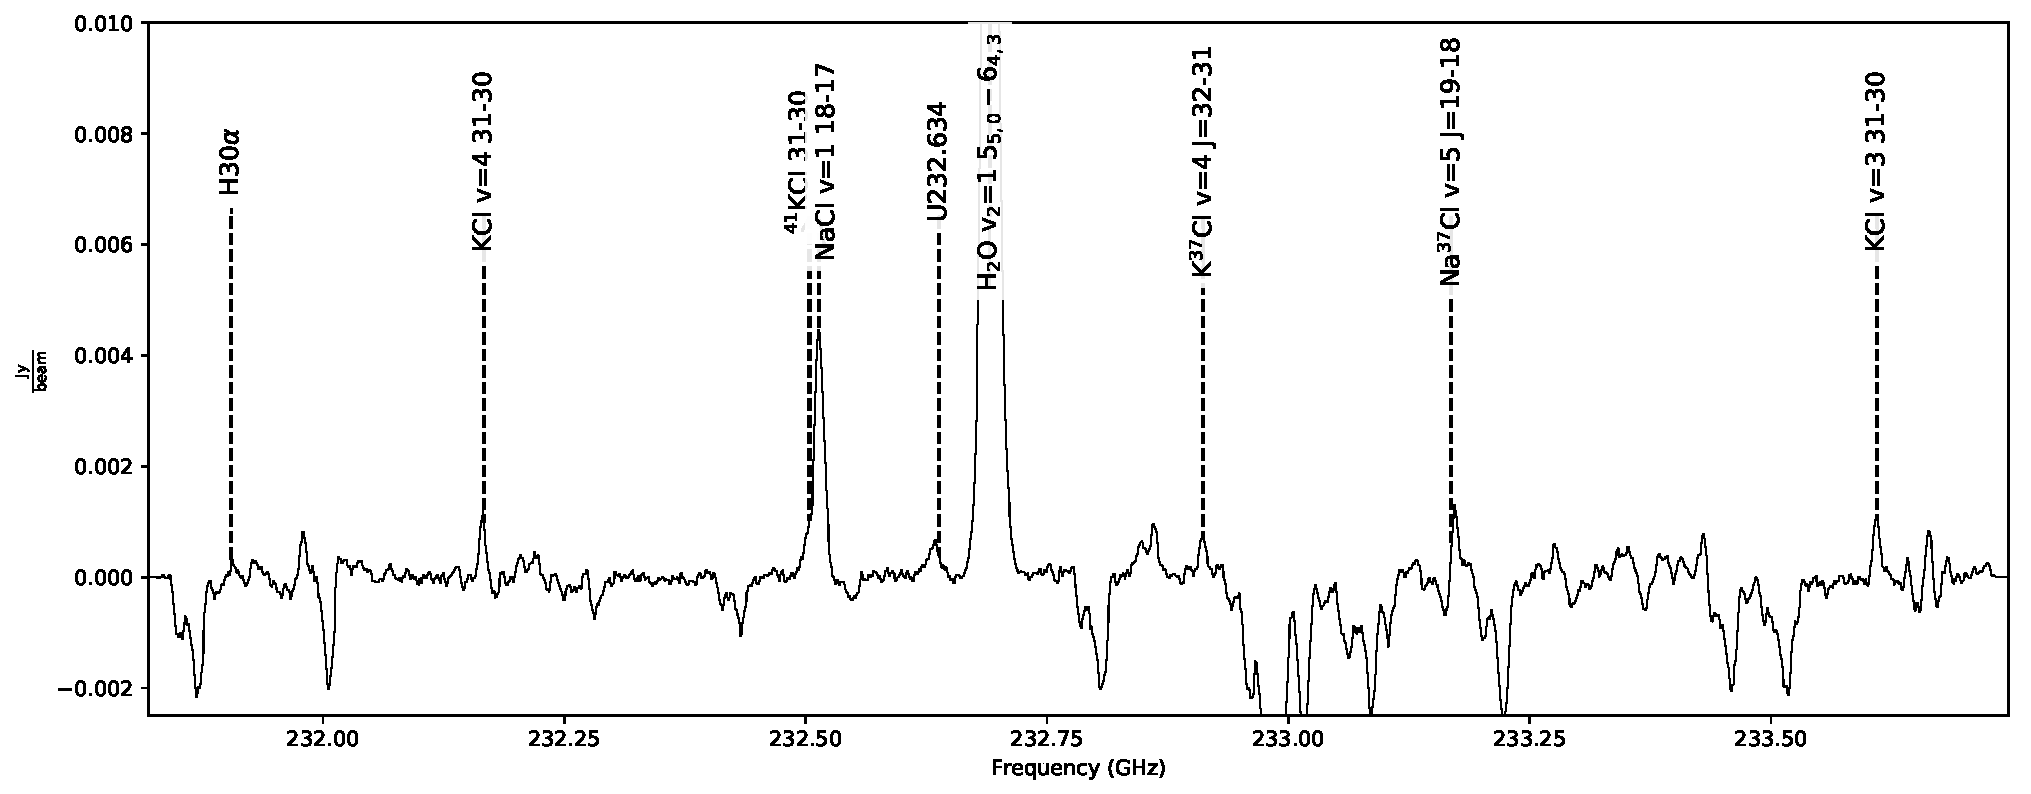
\includegraphics[scale=1,width=5.5in]{figures/lines_labeled_OrionSourceI_B6_spw1_robust0.5.pdf}
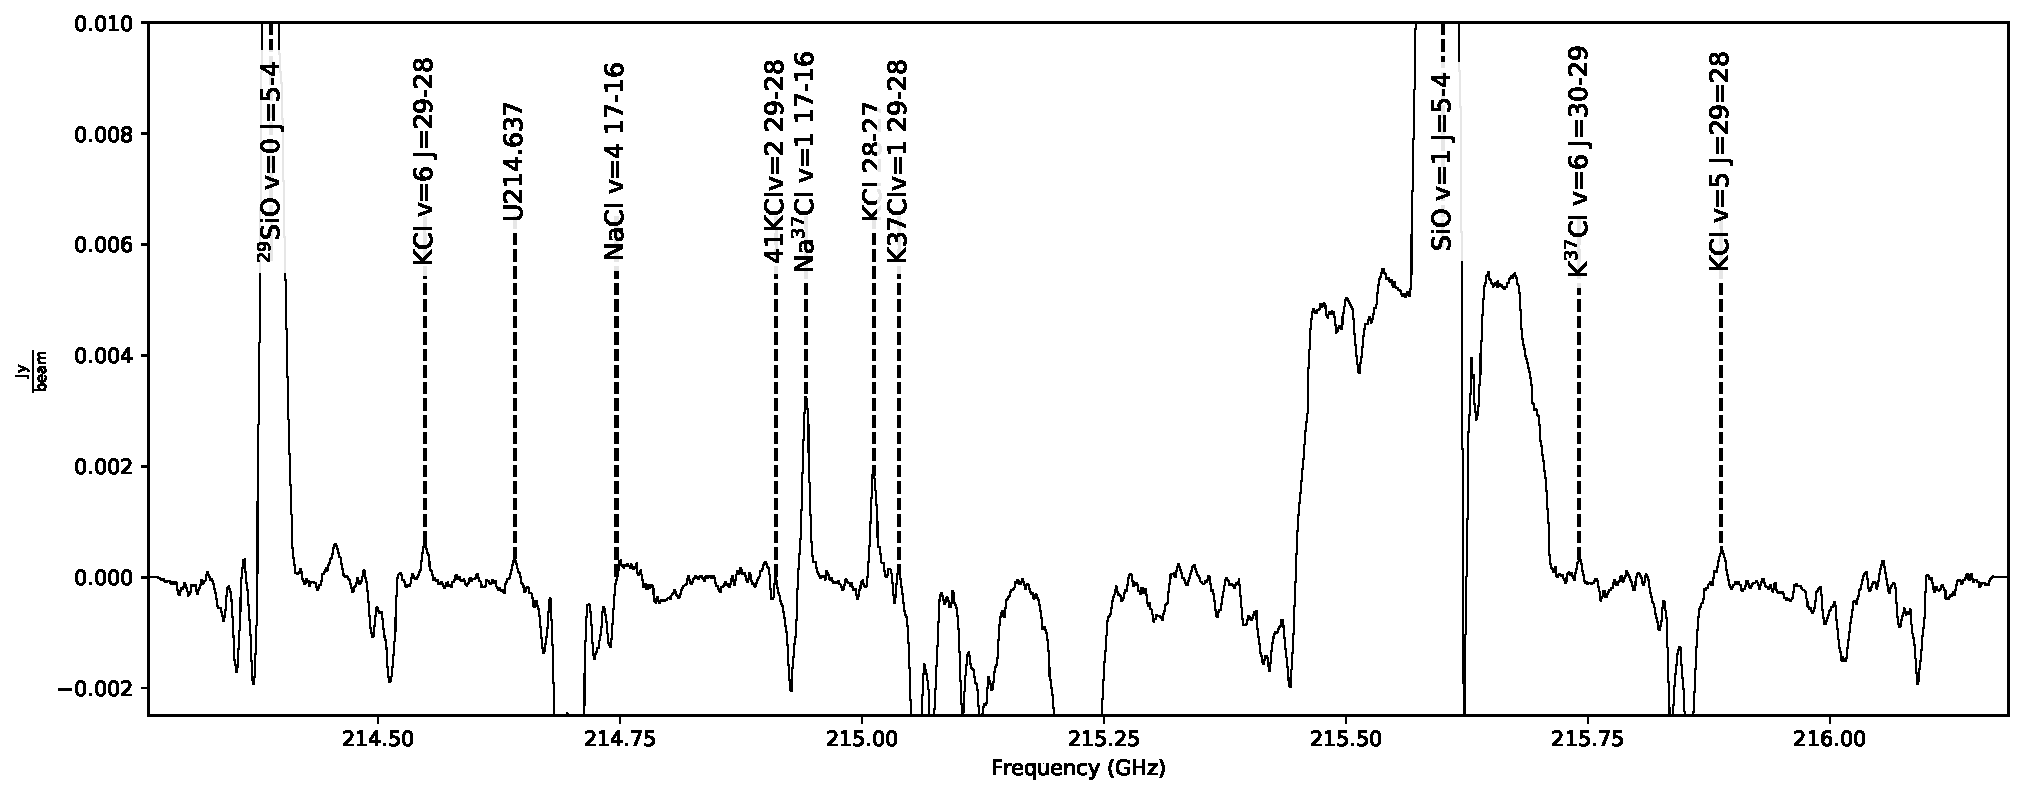
\includegraphics[scale=1,width=5.5in]{figures/lines_labeled_OrionSourceI_B6_spw2_robust0.5.pdf}
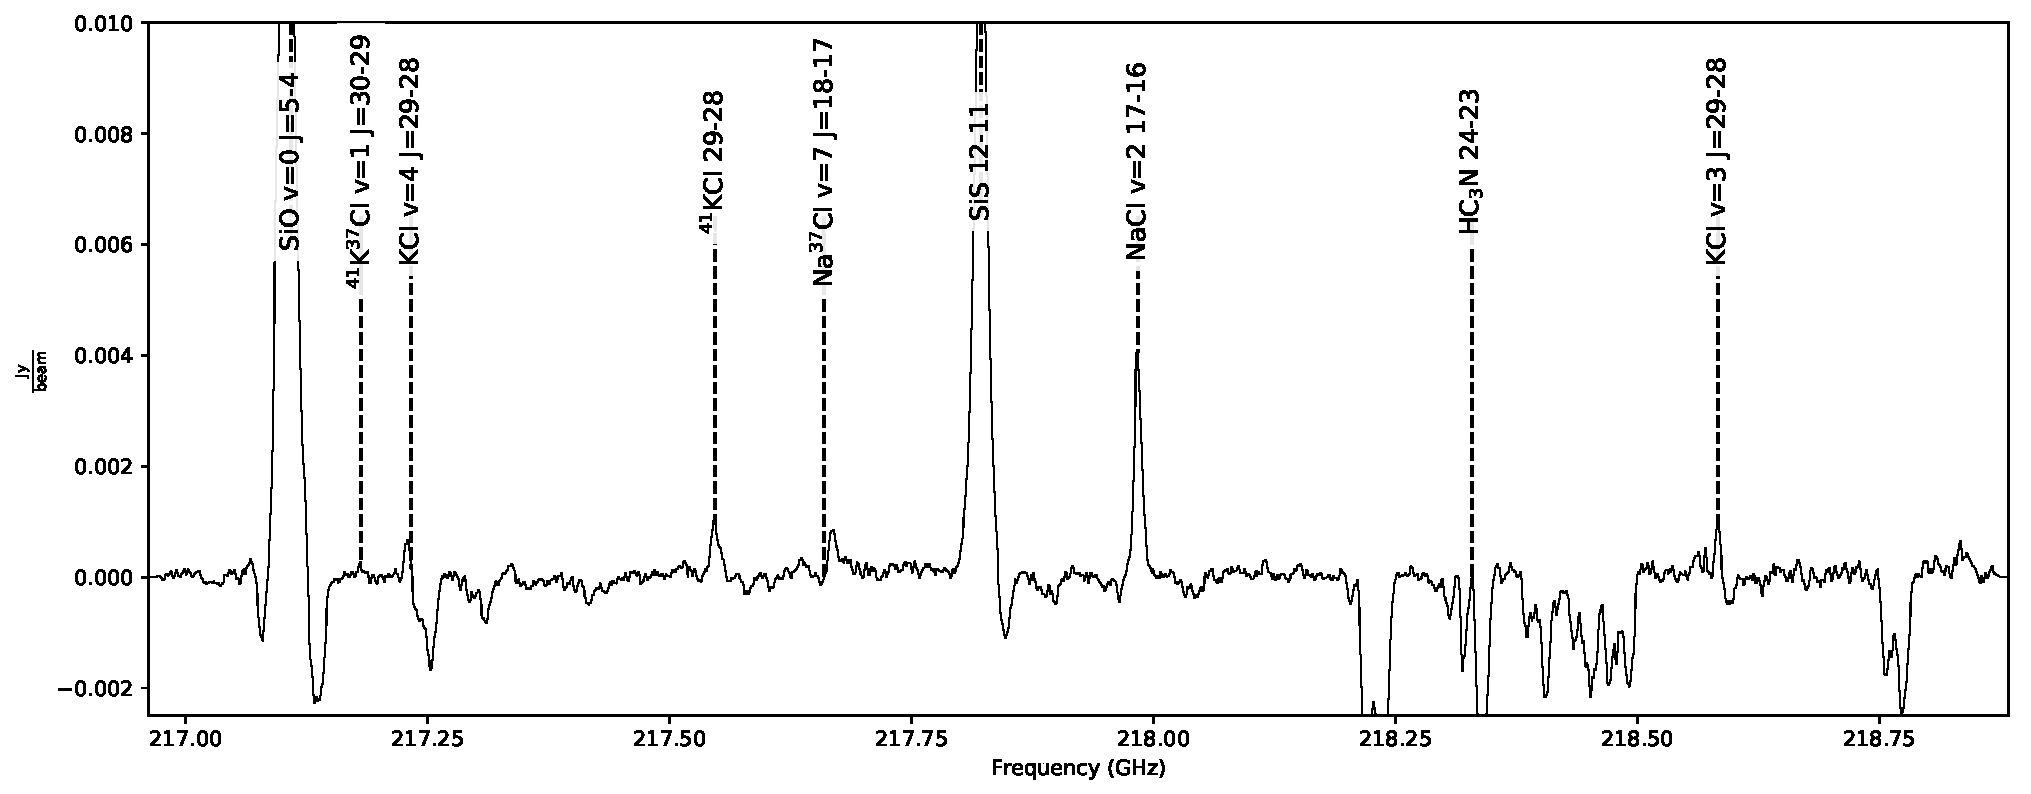
\includegraphics[scale=1,width=5.5in]{figures/lines_labeled_OrionSourceI_B6_spw3_robust0.5.pdf}
\caption{Stacked spectra B6}
\label{fig:spectrab6}
\end{figure*}
\begin{figure*}[!htp]
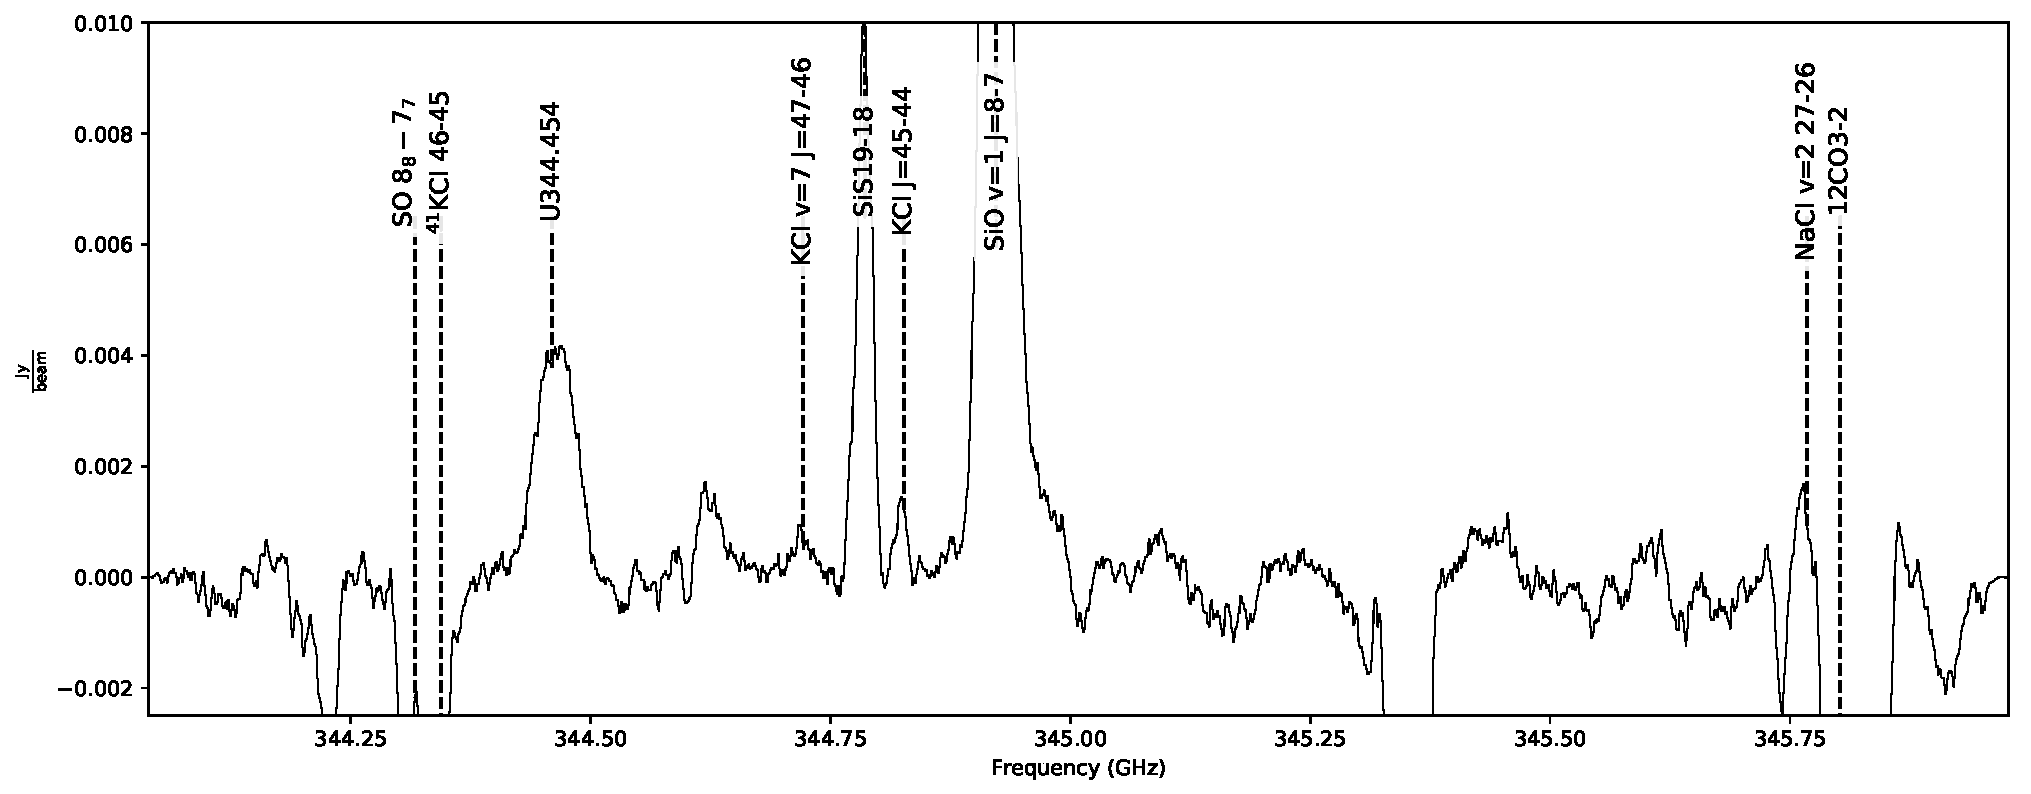
\includegraphics[scale=1,width=5.5in]{figures/lines_labeled_OrionSourceI_B7.lb_spw0_robust0.5.pdf}
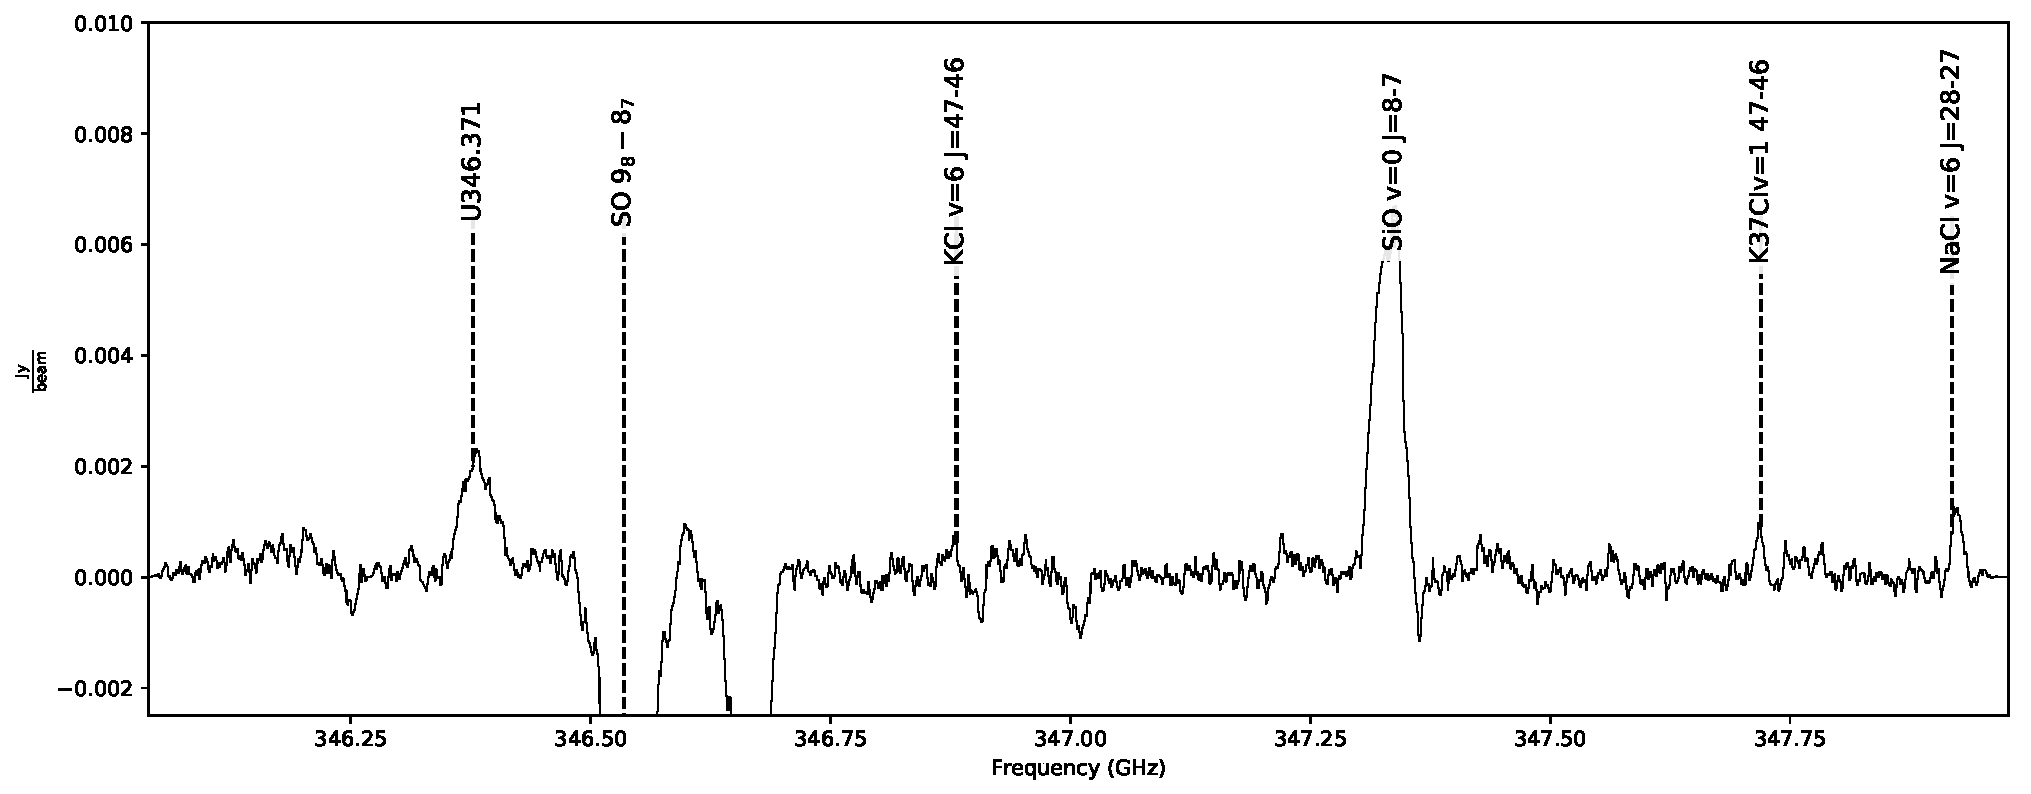
\includegraphics[scale=1,width=5.5in]{figures/lines_labeled_OrionSourceI_B7.lb_spw1_robust0.5.pdf}
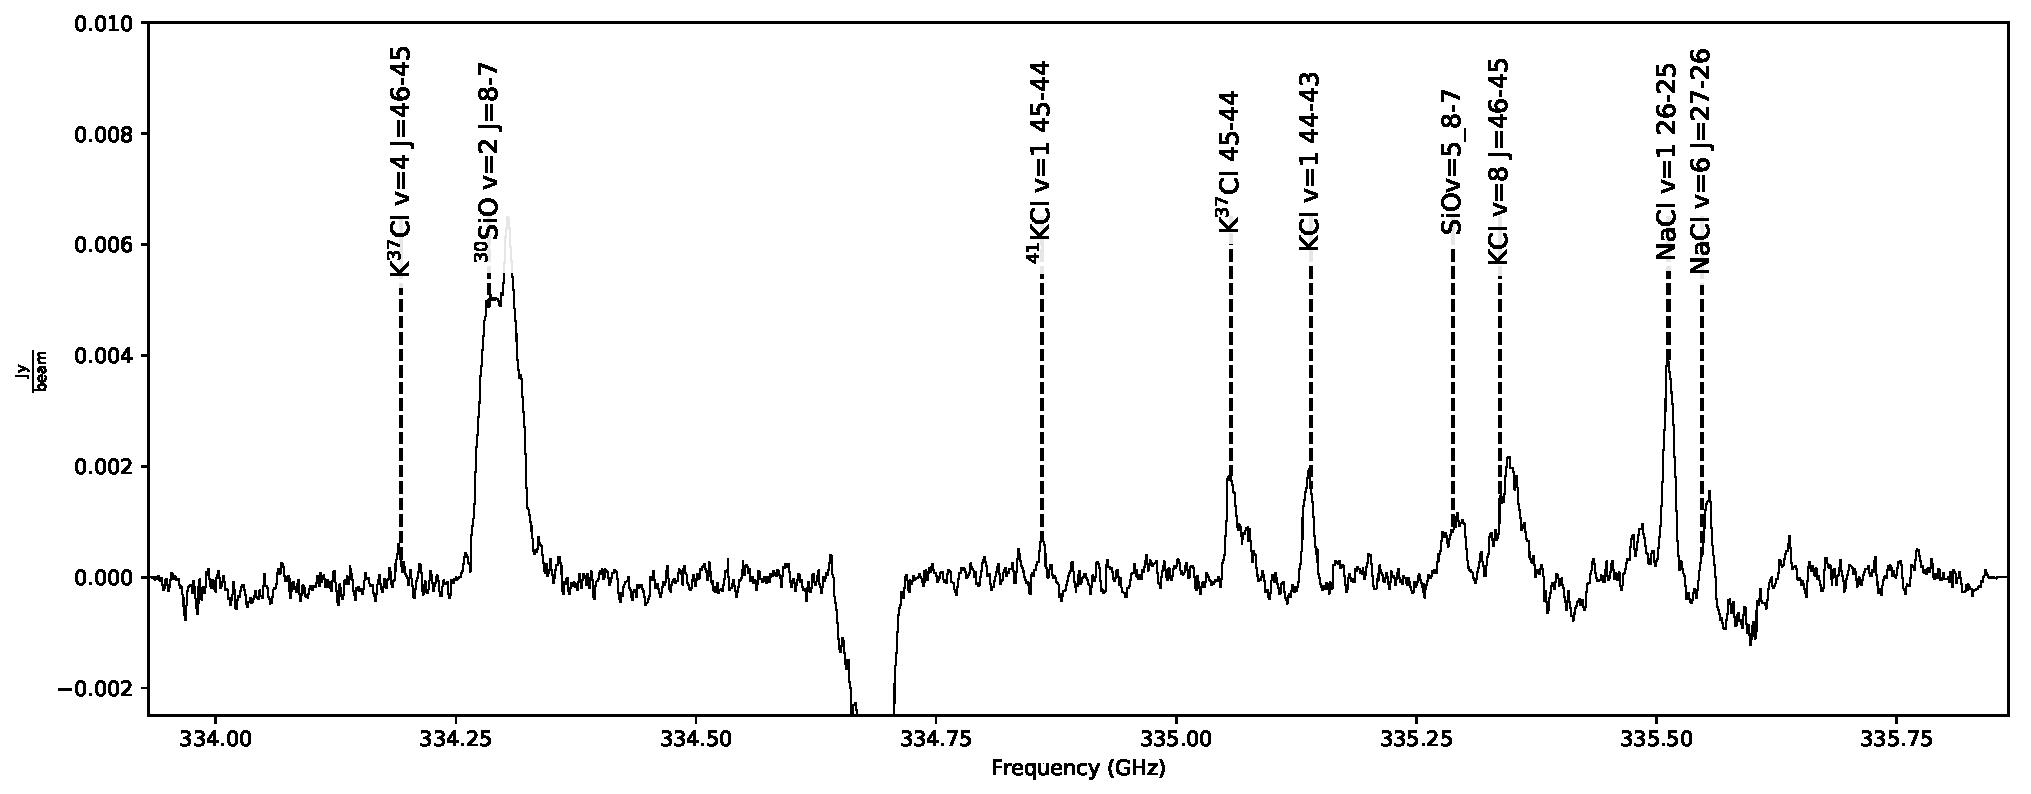
\includegraphics[scale=1,width=5.5in]{figures/lines_labeled_OrionSourceI_B7.lb_spw2_robust0.5.pdf}
\includegraphics[scale=1,width=5.5in]{figures/lines_labeled_OrionSourceI_B7.lb_spw3_robust0.5.pdf}
\caption{Stacked spectra B7}
\label{fig:spectrab7}
\end{figure*}


In Tables \ref{tab:all_detections_B3}-\ref{tab:all_detections_B7}, we report
all of the salt lines that are in our observable band and whether or not they were
detected.  We employ the following
flag scheme:
`d' for detection, `n' for nondetection, `q' for questionable (e.g., low
signal-to-noise, but possibly detected, or in regions where the noise is
not Gaussian and may be affected by other lines).
We additionally include a flag `c' for `confused', which we add to the flag
string if the line is blended with another brighter line of a different species.

Although transitions in higher vibrational states were measured, and some reported, in \citet{Caris2004a} and \citet{Caris2002a}, these did not provide the complete catalogs needed for this analysis, nor to our knowledge are these catalogues available in any of the standard online databases (i.e., CDMS, SLAIM, JPL {\color{red}TODO: cite
these}). We therefore used the predictions from the \citet{Barton2014a} catalog to identify lines with vibrational states $v>2$ for KCl and $v>4$ for NaCl.  In doing so, we found a systematic discrepancy in the rest frequencies
reported by \citet{Barton2014a} and those of \citet{Caris2004a} and \citet{Caris2002a}, and the  catalogs generated from them: the KCl lines appear to be systematically offset by $\sim$15-20 \kms.  The offset is a function of the vibrational
and rotational energy states, indicating that it resulted from an incorrect rotational
and/or distortion constant.  We correct for this error by performing a bilinear fit
in frequency as a function of $v_u$ and $J_u$.  In the transitions available
in both catalogs, the resulting offsets are generally $<0.1$ \kms, which is more than 
sufficient for a reliable match to our observational spectra.  We then applied these fitted models to the higher-$v$ states to get corrected rest frequencies.  A more detailed re-fitting and prediction of the frequencies is beyond the scope of this \emph{Letter}, but is certainly warranted for follow-up efforts.

% \textbf{\color{red} At the moment, all of the line frequencies are shifted
% to higher frequencies by 17 \kms (KCl) and 3 \kms (NaCl) because of a discrepancy
% between the \citep{Barton2014a} catalog line frequencies and those of CDMS,
% JPL, and SLAIM.  The latter three, catalogued in Splatalogue, agree, and they
% agree better with my measurements.}

\begin{table*}[htp]
\centering
\caption{All observed lines in Band 3}
\begin{tabular}{cccccccc}
\label{tab:all_detections_B3}
Species & v & J$_u$ & J$_l$ & E$_U$ & A$_{ul}$ & Frequency & Flag \\
\hline
$^{41}$K$^{35}$Cl & 8 & 12 & 11 & 3092.4 & 0.00041 & 85.80766 & -n \\
$^{23}$Na$^{35}$Cl & 8 & 7 & 6 & 4035.4 & 0.00031 & 85.87018 & -n \\
$^{39}$K$^{37}$Cl & 7 & 12 & 11 & 2713.3 & 0.00041 & 85.87379 & -n \\
$^{41}$K$^{37}$Cl & 3 & 12 & 11 & 1183.9 & 0.00039 & 85.93776 & -n \\
$^{23}$Na$^{37}$Cl & 5 & 7 & 6 & 2538.2 & 0.00030 & 85.98167 & -d \\
$^{41}$K$^{35}$Cl & 7 & 12 & 11 & 2720.7 & 0.00042 & 86.33986 & cn \\
$^{39}$K$^{37}$Cl & 6 & 12 & 11 & 2339.4 & 0.00041 & 86.40364 & -n \\
$^{41}$K$^{37}$Cl & 2 & 12 & 11 & 801.6 & 0.00039 & 86.45668 & -n \\
$^{23}$Na$^{35}$Cl & 7 & 7 & 6 & 3550.1 & 0.00031 & 86.51754 & -q \\
$^{23}$Na$^{37}$Cl & 4 & 7 & 6 & 2043.6 & 0.00030 & 86.62109 & -d \\
$^{39}$K$^{35}$Cl & 10 & 12 & 11 & 3869.7 & 0.00044 & 86.68041 & -n \\
$^{41}$K$^{35}$Cl & 6 & 12 & 11 & 2345.7 & 0.00042 & 86.87413 & -n \\
$^{39}$K$^{37}$Cl & 5 & 12 & 11 & 1962.2 & 0.00042 & 86.93553 & -n \\
$^{41}$K$^{37}$Cl & 1 & 12 & 11 & 416.1 & 0.00040 & 86.97743 & -q \\
$^{23}$Na$^{35}$Cl & 6 & 7 & 6 & 3060.0 & 0.00032 & 87.16921 & -d \\
$^{39}$K$^{35}$Cl & 9 & 12 & 11 & 3500.3 & 0.00044 & 87.22792 & -n \\
$^{23}$Na$^{37}$Cl & 3 & 7 & 6 & 1544.3 & 0.00030 & 87.26464 & -d \\
$^{41}$K$^{35}$Cl & 5 & 12 & 11 & 1967.6 & 0.00042 & 87.41041 & -n \\
$^{39}$K$^{37}$Cl & 4 & 12 & 11 & 1581.9 & 0.00042 & 87.46938 & -n \\
$^{41}$K$^{37}$Cl & 0 & 12 & 11 & 27.3 & 0.00040 & 87.50010 & -q \\
$^{39}$K$^{35}$Cl & 8 & 12 & 11 & 3127.7 & 0.00044 & 87.77742 & -n \\
$^{23}$Na$^{35}$Cl & 5 & 7 & 6 & 2565.2 & 0.00032 & 87.82519 & -d \\
$^{23}$Na$^{37}$Cl & 2 & 7 & 6 & 1040.1 & 0.00031 & 87.91232 & -d \\
$^{41}$K$^{35}$Cl & 4 & 12 & 11 & 1586.3 & 0.00043 & 87.94866 & -n \\
$^{39}$K$^{37}$Cl & 3 & 12 & 11 & 1198.3 & 0.00042 & 88.00523 & -d \\
$^{39}$K$^{35}$Cl & 7 & 12 & 11 & 2751.8 & 0.00045 & 88.32895 & -q \\
$^{23}$Na$^{35}$Cl & 4 & 7 & 6 & 2065.5 & 0.00032 & 88.48549 & -d \\
$^{41}$K$^{35}$Cl & 3 & 12 & 11 & 1201.7 & 0.00043 & 88.48896 & cq \\
$^{39}$K$^{37}$Cl & 2 & 12 & 11 & 811.5 & 0.00042 & 88.54307 & -d \\
$^{23}$Na$^{37}$Cl & 1 & 7 & 6 & 531.1 & 0.00031 & 88.56415 & -d \\
$^{39}$K$^{35}$Cl & 6 & 12 & 11 & 2372.8 & 0.00045 & 88.88253 & -n \\
$^{41}$K$^{35}$Cl & 2 & 12 & 11 & 813.8 & 0.00043 & 89.03129 & -d \\
$^{39}$K$^{37}$Cl & 1 & 12 & 11 & 421.4 & 0.00043 & 89.08292 & -d \\
$^{23}$Na$^{35}$Cl & 3 & 7 & 6 & 1561.0 & 0.00033 & 89.15011 & -d \\
$^{41}$K$^{37}$Cl & 10 & 13 & 12 & 3776.8 & 0.00048 & 89.21871 & -n \\
$^{23}$Na$^{37}$Cl & 0 & 7 & 6 & 17.1 & 0.00031 & 89.22011 & -d \\
$^{39}$K$^{35}$Cl & 4 & 13 & 12 & 1609.5 & 0.00058 & 97.49133 & -d \\
$^{23}$Na$^{37}$Cl & 6 & 8 & 7 & 3032.7 & 0.00045 & 97.53449 & -q \\
$^{41}$K$^{35}$Cl & 0 & 13 & 12 & 32.8 & 0.00056 & 97.62809 & -d \\
$^{41}$K$^{37}$Cl & 7 & 14 & 13 & 2690.7 & 0.00061 & 97.85364 & -n \\
$^{39}$K$^{35}$Cl & 3 & 13 & 12 & 1220.6 & 0.00059 & 98.09753 & -d \\
$^{23}$Na$^{35}$Cl & 8 & 8 & 7 & 4040.1 & 0.00047 & 98.13295 & -q \\
$^{23}$Na$^{37}$Cl & 5 & 8 & 7 & 2542.9 & 0.00045 & 98.26052 & -q \\
$^{39}$K$^{37}$Cl & 10 & 14 & 13 & 3825.5 & 0.00064 & 98.33904 & -n \\
$^{41}$K$^{37}$Cl & 6 & 14 & 13 & 2321.0 & 0.00061 & 98.44993 & -n \\
$^{39}$K$^{35}$Cl & 2 & 13 & 12 & 828.3 & 0.00059 & 98.70595 & -d \\
$^{41}$K$^{35}$Cl & 10 & 14 & 13 & 3835.7 & 0.00065 & 98.86759 & cn \\
$^{23}$Na$^{35}$Cl & 7 & 8 & 7 & 3554.8 & 0.00047 & 98.87277 & -q \\
$^{39}$K$^{37}$Cl & 9 & 14 & 13 & 3461.0 & 0.00065 & 98.94969 & -n \\
$^{23}$Na$^{37}$Cl & 4 & 8 & 7 & 2048.4 & 0.00045 & 98.99127 & -d \\
$^{41}$K$^{37}$Cl & 5 & 14 & 13 & 1948.2 & 0.00062 & 99.04845 & -n \\
$^{39}$K$^{35}$Cl & 1 & 13 & 12 & 432.6 & 0.00059 & 99.31663 & -d \\
$^{41}$K$^{35}$Cl & 9 & 14 & 13 & 3470.3 & 0.00066 & 99.48329 & -n \\
$^{39}$K$^{37}$Cl & 8 & 14 & 13 & 3093.3 & 0.00065 & 99.56276 & -n \\
$^{23}$Na$^{35}$Cl & 6 & 8 & 7 & 3064.8 & 0.00048 & 99.61753 & -d \\
$^{41}$K$^{37}$Cl & 4 & 14 & 13 & 1572.3 & 0.00062 & 99.64924 & -n \\
$^{23}$Na$^{37}$Cl & 3 & 8 & 7 & 1549.1 & 0.00046 & 99.72675 & -d \\
$^{39}$K$^{35}$Cl & 0 & 13 & 12 & 33.6 & 0.00060 & 99.92952 & -d \\
$^{41}$K$^{35}$Cl & 8 & 14 & 13 & 3101.7 & 0.00066 & 100.10138 & -n \\
$^{39}$K$^{37}$Cl & 7 & 14 & 13 & 2722.6 & 0.00065 & 100.17822 & -n \\
$^{41}$K$^{37}$Cl & 3 & 14 & 13 & 1193.2 & 0.00063 & 100.25229 & -n \\
$^{23}$Na$^{35}$Cl & 5 & 8 & 7 & 2570.0 & 0.00048 & 100.36722 & -d \\
$^{23}$Na$^{37}$Cl & 2 & 8 & 7 & 1045.0 & 0.00046 & 100.46695 & -d \\
$^{41}$K$^{35}$Cl & 7 & 14 & 13 & 2730.0 & 0.00067 & 100.72190 & -n \\
$^{39}$K$^{37}$Cl & 6 & 14 & 13 & 2348.7 & 0.00066 & 100.79603 & -q \\
$^{41}$K$^{37}$Cl & 2 & 14 & 13 & 810.9 & 0.00063 & 100.85758 & -n \\
$^{39}$K$^{35}$Cl & 10 & 14 & 13 & 3879.0 & 0.00070 & 101.12088 & -n \\
$^{23}$Na$^{35}$Cl & 4 & 8 & 7 & 2070.4 & 0.00048 & 101.12183 & -d \\
$^{23}$Na$^{37}$Cl & 1 & 8 & 7 & 536.0 & 0.00047 & 101.21188 & -d \\
\hline
\end{tabular}

\par 
\end{table*}

\begin{table*}[htp]
\centering
\caption{All detected lines in Band 6}
\begin{tabular}{ccccccc}
\label{tab:all_detections_B6}
Species & v & J$_u$ & J$_l$ & E$_U$ & Frequency & Flag \\
\hline
$^{39}$K$^{37}$Cl & 7 & 30 & 29 & 2846.1 & 214.41527 & -n \\
$^{23}$Na$^{37}$Cl & 9 & 18 & 17 & 4547.4 & 214.43575 & cn \\
$^{39}$K$^{35}$Cl & 6 & 29 & 28 & 2499.6 & 214.54412 & -d \\
$^{41}$K$^{37}$Cl & 3 & 30 & 29 & 1316.8 & 214.57918 & -n \\
$^{23}$Na$^{35}$Cl & 4 & 17 & 16 & 2139.6 & 214.74036 & cn \\
$^{41}$K$^{35}$Cl & 2 & 29 & 28 & 940.8 & 214.90740 & cq \\
$^{23}$Na$^{37}$Cl & 1 & 17 & 16 & 606.5 & 214.93872 & -d \\
$^{39}$K$^{35}$Cl & 0 & 28 & 27 & 149.7 & 215.00828 & -d \\
$^{39}$K$^{37}$Cl & 1 & 29 & 28 & 548.5 & 215.03464 & cq \\
$^{41}$K$^{37}$Cl & 8 & 31 & 30 & 3187.6 & 215.09368 & cn \\
$^{41}$K$^{35}$Cl & 7 & 30 & 29 & 2854.2 & 215.57755 & cn \\
$^{39}$K$^{37}$Cl & 6 & 30 & 29 & 2473.0 & 215.73679 & -d \\
$^{41}$K$^{37}$Cl & 2 & 30 & 29 & 935.3 & 215.87559 & -n \\
$^{39}$K$^{35}$Cl & 5 & 29 & 28 & 2118.0 & 215.88373 & -d \\
$^{23}$Na$^{37}$Cl & 8 & 18 & 17 & 4072.5 & 216.04057 & -n \\
$^{39}$K$^{37}$Cl & 5 & 30 & 29 & 2096.7 & 217.06391 & -q \\
$^{41}$K$^{37}$Cl & 1 & 30 & 29 & 550.6 & 217.17723 & -q \\
$^{39}$K$^{35}$Cl & 4 & 29 & 28 & 1733.2 & 217.22891 & cd \\
$^{23}$Na$^{35}$Cl & 10 & 18 & 17 & 5070.5 & 217.31725 & cn \\
$^{39}$K$^{37}$Cl & 10 & 31 & 30 & 3957.2 & 217.47744 & -n \\
$^{41}$K$^{35}$Cl & 0 & 29 & 28 & 156.7 & 217.54317 & -d \\
$^{23}$Na$^{37}$Cl & 7 & 18 & 17 & 3593.1 & 217.65560 & -q \\
$^{41}$K$^{37}$Cl & 6 & 31 & 30 & 2452.9 & 217.72366 & -n \\
$^{39}$K$^{35}$Cl & 9 & 30 & 29 & 3635.2 & 217.79704 & cn \\
$^{23}$Na$^{35}$Cl & 2 & 17 & 16 & 1127.5 & 217.97998 & -d \\
$^{41}$K$^{35}$Cl & 5 & 30 & 29 & 2102.8 & 218.24805 & -n \\
$^{39}$K$^{37}$Cl & 4 & 30 & 29 & 1717.2 & 218.39657 & cn \\
$^{41}$K$^{37}$Cl & 0 & 30 & 29 & 162.6 & 218.48414 & cn \\
$^{39}$K$^{35}$Cl & 3 & 29 & 28 & 1345.1 & 218.57971 & -d \\
$^{41}$K$^{35}$Cl & 10 & 31 & 30 & 3968.1 & 218.64471 & -n \\
$^{39}$K$^{37}$Cl & 9 & 31 & 30 & 3593.5 & 218.82568 & -q \\
$^{23}$Na$^{37}$Cl & 0 & 18 & 17 & 104.6 & 229.24601 & -d \\
$^{39}$K$^{35}$Cl & 6 & 31 & 30 & 2521.2 & 229.29217 & cd \\
$^{23}$Na$^{35}$Cl & 10 & 19 & 18 & 5081.5 & 229.36540 & cn \\
$^{41}$K$^{35}$Cl & 2 & 31 & 30 & 962.5 & 229.68227 & cd \\
$^{23}$Na$^{37}$Cl & 7 & 19 & 18 & 3604.1 & 229.72316 & cn \\
$^{39}$K$^{37}$Cl & 1 & 31 & 30 & 570.2 & 229.81880 & -d \\
$^{41}$K$^{35}$Cl & 7 & 32 & 31 & 2875.9 & 229.90046 & -q \\
$^{39}$K$^{37}$Cl & 6 & 32 & 31 & 2494.7 & 230.07072 & -d \\
$^{41}$K$^{37}$Cl & 2 & 32 & 31 & 957.1 & 230.22070 & -q \\
$^{41}$K$^{37}$Cl & 7 & 33 & 32 & 2843.6 & 230.31852 & cn \\
$^{39}$K$^{35}$Cl & 0 & 30 & 29 & 171.4 & 230.32064 & -d \\
$^{39}$K$^{35}$Cl & 5 & 31 & 30 & 2139.8 & 230.72399 & -d \\
$^{23}$Na$^{35}$Cl & 2 & 18 & 17 & 1138.6 & 230.77883 & -d \\
$^{39}$K$^{35}$Cl & 10 & 32 & 31 & 4025.6 & 230.81309 & -n \\
$^{39}$K$^{35}$Cl & 4 & 31 & 30 & 1755.1 & 232.16185 & -d \\
$^{39}$K$^{35}$Cl & 9 & 32 & 31 & 3657.1 & 232.26613 & cn \\
$^{41}$K$^{35}$Cl & 0 & 31 & 30 & 178.7 & 232.49980 & cn \\
$^{23}$Na$^{35}$Cl & 1 & 18 & 17 & 625.2 & 232.50998 & -d \\
$^{41}$K$^{35}$Cl & 10 & 33 & 32 & 3990.1 & 232.69933 & cn \\
$^{41}$K$^{35}$Cl & 5 & 32 & 31 & 2124.8 & 232.74872 & -q \\
$^{23}$Na$^{35}$Cl & 8 & 19 & 18 & 4127.2 & 232.84920 & -q \\
$^{39}$K$^{37}$Cl & 9 & 33 & 32 & 3615.5 & 232.89230 & -n \\
$^{39}$K$^{37}$Cl & 4 & 32 & 31 & 1739.2 & 232.90755 & -d \\
$^{41}$K$^{37}$Cl & 10 & 34 & 33 & 3942.7 & 232.97243 & cn \\
$^{41}$K$^{37}$Cl & 0 & 32 & 31 & 184.6 & 233.00319 & cn \\
$^{41}$K$^{37}$Cl & 5 & 33 & 32 & 2102.9 & 233.12954 & cn \\
$^{23}$Na$^{37}$Cl & 5 & 19 & 18 & 2631.4 & 233.16458 & cd \\
$^{39}$K$^{35}$Cl & 3 & 31 & 30 & 1367.1 & 233.60570 & -d \\
$^{39}$K$^{35}$Cl & 8 & 32 & 31 & 3285.5 & 233.72540 & -n \\
\hline
\end{tabular}

\par 
\end{table*}

\begin{table*}[htp]
\centering
% \caption{All observed lines in Band 7}
% "observed" often means "detected", hence is misleading - Dick
\caption{Salt lines in Band 7}
\begin{tabular}{cccccccc}
\label{tab:all_detections_B7}
Species & v & J$_u$ & J$_l$ & E$_U$ & A$_{ul}$ & Frequency & Flag \\
\hline
$^{39}$K$^{37}$Cl & 5 & 46 & 45 & 2310.3 & 0.02398 & 332.14436 & cn \\
$^{39}$K$^{35}$Cl & 6 & 45 & 44 & 2712.4 & 0.02429 & 332.22193 & cq \\
$^{41}$K$^{37}$Cl & 8 & 48 & 47 & 3413.8 & 0.02483 & 332.29761 & -n \\
$^{41}$K$^{37}$Cl & 1 & 46 & 45 & 764.4 & 0.02295 & 332.34847 & -n \\
$^{41}$K$^{35}$Cl & 2 & 45 & 44 & 1154.0 & 0.02331 & 332.81369 & -n \\
$^{41}$K$^{35}$Cl & 9 & 47 & 46 & 3818.5 & 0.02527 & 332.83163 & -n \\
$^{23}$Na$^{35}$Cl & 2 & 26 & 25 & 1250.2 & 0.01800 & 333.00729 & -d \\
$^{39}$K$^{37}$Cl & 1 & 45 & 44 & 761.8 & 0.02309 & 333.01833 & cn \\
$^{23}$Na$^{35}$Cl & 7 & 27 & 26 & 3757.5 & 0.01900 & 333.03612 & cq \\
$^{39}$K$^{35}$Cl & 2 & 44 & 43 & 1155.3 & 0.02336 & 333.06770 & -d \\
$^{39}$K$^{37}$Cl & 8 & 47 & 46 & 3441.9 & 0.02504 & 333.10414 & -n \\
$^{39}$K$^{35}$Cl & 9 & 46 & 45 & 3849.6 & 0.02539 & 333.23510 & -n \\
$^{41}$K$^{37}$Cl & 4 & 47 & 46 & 1921.1 & 0.02398 & 333.43025 & -n \\
$^{23}$Na$^{37}$Cl & 4 & 27 & 26 & 2251.3 & 0.01800 & 333.45906 & -d \\
$^{41}$K$^{35}$Cl & 5 & 46 & 45 & 2317.6 & 0.02438 & 333.95245 & -n \\
$^{39}$K$^{37}$Cl & 4 & 46 & 45 & 1932.1 & 0.02415 & 334.18696 & -n \\
$^{39}$K$^{35}$Cl & 5 & 45 & 44 & 2332.2 & 0.02446 & 334.29930 & -d \\
$^{41}$K$^{37}$Cl & 7 & 48 & 47 & 3049.3 & 0.02501 & 334.32791 & cd \\
$^{41}$K$^{37}$Cl & 0 & 46 & 45 & 377.7 & 0.02311 & 334.35249 & cn \\
$^{41}$K$^{35}$Cl & 1 & 45 & 44 & 764.9 & 0.02347 & 334.85439 & -d \\
$^{41}$K$^{35}$Cl & 8 & 47 & 46 & 3452.1 & 0.02545 & 334.89960 & -n \\
$^{41}$K$^{37}$Cl & 10 & 49 & 48 & 4149.6 & 0.02605 & 335.04657 & cn \\
$^{39}$K$^{37}$Cl & 0 & 45 & 44 & 370.4 & 0.02325 & 335.05072 & -d \\
$^{39}$K$^{35}$Cl & 1 & 44 & 43 & 761.7 & 0.02353 & 335.13396 & -d \\
$^{39}$K$^{37}$Cl & 7 & 47 & 46 & 3073.3 & 0.02522 & 335.16416 & -q \\
$^{39}$K$^{35}$Cl & 8 & 46 & 45 & 3479.1 & 0.02557 & 335.33093 & cq \\
$^{41}$K$^{37}$Cl & 3 & 47 & 46 & 1544.2 & 0.02414 & 335.45237 & -n \\
$^{23}$Na$^{35}$Cl & 1 & 26 & 25 & 737.2 & 0.01800 & 335.50656 & -d \\
$^{23}$Na$^{35}$Cl & 6 & 27 & 26 & 3269.0 & 0.01900 & 335.54793 & cq \\
$^{23}$Na$^{37}$Cl & 8 & 28 & 27 & 4211.3 & 0.02000 & 335.63074 & cn \\
$^{41}$K$^{35}$Cl & 7 & 48 & 47 & 3099.1 & 0.02730 & 344.08981 & cn \\
$^{41}$K$^{35}$Cl & 0 & 46 & 45 & 389.0 & 0.02525 & 344.33834 & cn \\
$^{39}$K$^{37}$Cl & 6 & 48 & 47 & 2718.1 & 0.02705 & 344.35234 & cn \\
$^{41}$K$^{37}$Cl & 2 & 48 & 47 & 1180.5 & 0.02589 & 344.60998 & cq \\
$^{39}$K$^{35}$Cl & 7 & 47 & 46 & 3122.1 & 0.02747 & 344.71476 & -d \\
$^{41}$K$^{35}$Cl & 10 & 49 & 48 & 4214.6 & 0.02843 & 344.73191 & -n \\
$^{39}$K$^{35}$Cl & 0 & 45 & 44 & 381.2 & 0.02534 & 344.82061 & -d \\
$^{39}$K$^{37}$Cl & 9 & 49 & 48 & 3840.1 & 0.02817 & 345.02524 & -n \\
$^{23}$Na$^{35}$Cl & 7 & 28 & 27 & 3774.1 & 0.02100 & 345.31422 & cn \\
$^{41}$K$^{35}$Cl & 3 & 47 & 46 & 1572.6 & 0.02637 & 345.37541 & cn \\
$^{41}$K$^{37}$Cl & 5 & 49 & 48 & 2327.8 & 0.02698 & 345.40918 & cn \\
$^{39}$K$^{35}$Cl & 10 & 48 & 47 & 4249.6 & 0.02864 & 345.42961 & cn \\
$^{39}$K$^{37}$Cl & 2 & 47 & 46 & 1182.6 & 0.02612 & 345.59885 & cn \\
$^{23}$Na$^{37}$Cl & 4 & 28 & 27 & 2267.9 & 0.02000 & 345.75480 & cn \\
$^{23}$Na$^{35}$Cl & 2 & 27 & 26 & 1266.8 & 0.02000 & 345.76204 & cd \\
$^{39}$K$^{35}$Cl & 3 & 46 & 45 & 1578.4 & 0.02650 & 345.94809 & cn \\
$^{41}$K$^{35}$Cl & 6 & 48 & 47 & 2726.5 & 0.02750 & 346.22022 & -n \\
$^{39}$K$^{37}$Cl & 5 & 48 & 47 & 2343.3 & 0.02724 & 346.47449 & -n \\
$^{41}$K$^{37}$Cl & 1 & 48 & 47 & 797.3 & 0.02607 & 346.69248 & cn \\
$^{39}$K$^{35}$Cl & 6 & 47 & 46 & 2745.3 & 0.02767 & 346.87489 & -d \\
$^{41}$K$^{35}$Cl & 9 & 49 & 48 & 3851.5 & 0.02863 & 346.87825 & cn \\
$^{39}$K$^{37}$Cl & 8 & 49 & 48 & 3474.8 & 0.02837 & 347.16340 & -n \\
$^{41}$K$^{35}$Cl & 2 & 47 & 46 & 1187.0 & 0.02655 & 347.49773 & -q \\
$^{41}$K$^{37}$Cl & 4 & 49 & 48 & 1954.1 & 0.02717 & 347.50839 & -n \\
$^{23}$Na$^{37}$Cl & 8 & 29 & 28 & 4228.0 & 0.02200 & 347.55955 & -n \\
$^{39}$K$^{35}$Cl & 9 & 48 & 47 & 3882.6 & 0.02884 & 347.60673 & -n \\
$^{39}$K$^{37}$Cl & 1 & 47 & 46 & 794.8 & 0.02630 & 347.71265 & -d \\
$^{23}$Na$^{35}$Cl & 6 & 28 & 27 & 3285.7 & 0.02100 & 347.91891 & nc \\
\hline
\end{tabular}

\par 
\end{table*}


%The low observed brightness temperatures suggest that the emission from
%these lines is optically thin.




\section{Discussion}
NaCl and KCl have only been seen in a small handful of other sources,
all of which were moderately high-mass evolved stars blowing off their envelopes.
The known detections include the carbon star envelope IRC +10216 \citep{Cernicharo1987a,Agundez2012a},
the post-AGB star envelope CRL 2688 \citep{Highberger2003a}, and the oxygen-rich
evolved star envelopes of VY Canis Majoris and IK Tauri \citep{Milam2007a}. To our knowledge, 
\sourcei is only the 5th astronomical source in which KCl and NaCl have been
detected.
However, there were no detections of vibrationally excited NaCl or KCl in any
of the previous observations,
% (\citealt{Agundez2012a} presented the most systematic study of salt lines, 
%which only included detections of v=0 rotational transitions),
while \sourcei exhibits clear emission up to v=6 in both NaCl and KCl.

In these evolved stars, v=0 rotational transitions of NaCl were observed
with rotational temperatures ${T_{rot}\sim70-100}$ K (IK Tau, VY CMa), inferred
local temperatures of $\sim200$ K in shocks (CRL 2688), and $T\approx700$ K  in
an expanding shell (IRC+10216).  Below, we attempt to determine the physical
conditions in the \sourcei salt emission regions.
% Carbon star envelope IRC +10216, d ~ 170 pc
% CRL2688 post-AGB * \citep{Highberger2003a} ~ 1 kpc
% IK Tauri, VY Canis Majoris \citep{Milam2007a}

\subsection{Where is the emission coming from?}
In \sourcei, the salt lines originate from the surface layers of the disk,
% \citet{Ginsburg2018b} showed that these species come only from the disk's
% immediate surroundings, 
unlike SiO and \water that both exhibit high vertical
extents consistent with outflow \citep{Ginsburg2018b}.  No emission in the salt lines is observed
toward the optically thick continuum in the disk midplane (Figure \ref{fig:spatial}).
\citet{Ginsburg2018b} modeled the salt line emission as a truncated Keplerian
disk, finding that the radial distribution of the emission has an inner cutoff
$\approx35-40$ AU and an outer cutoff $\approx55-60$ AU.

% ((constants.sigma_sb * 4 * np.pi * (35*u.au)**2 / (1e4*u.L_sun))**(-1/4)).decompose()
% <Quantity 665.33595877 K>
% ((constants.sigma_sb * 4 * np.pi * (60*u.au)**2 / (1e4*u.L_sun))**(-1/4)).decompose()
% <Quantity 508.15873227 K>
The equilibrium temperature in this radius range can be computed assuming the central
source has a luminosity $L=10^4 \lsun = 4 \pi r^2 \sigma_{SB} T^4 $, where we
solve for temperature with $r$ at the inner and outer radius, giving $T_{eq} =
508-665$ K for $r=35-60$ AU, assuming the disk intercepts all of the starlight 
at this radius.  More realistically, providing the opposite limiting case,
$T_{eq}=120-185$ K for a flat disk \citep{Chiang1997a}.  These cooler temperatures
are consistent with the observed brightness temperatures in the outer
part of the continuum disk (in Figure \ref{fig:spatial}, the NaCl emission
begins just beyond the $T=300$ K contour), although temperature in the inner
portion of the disk reaches $\gtrsim500$ K.

\begin{figure*}[!htp]
\includegraphics[scale=1,width=2.25in]{figures/OrionSourceI_NaClv=3_7-6_robust0.5.maskedclarkclean10000_medsub_K_peak_offset_contours.pdf}
\includegraphics[scale=1,width=2.25in]{figures/OrionSourceI_NaClv=1_18-17_robust0.5.maskedclarkclean10000_medsub_K_peak_offset_contours.pdf}
\includegraphics[scale=1,width=2.25in]{figures/OrionSourceI_NaClv=2_26-25_robust0.5.maskedclarkclean10000_medsub_K_peak_offset_contours.pdf}
\caption{Peak intensity images of NaCl lines in each band showing the spatial
distribution of the emission.  From left to right, the lines are: 87.26 GHz
NaCl v=3 J=7-6, 232.51 GHz NaCl v=1 J=18-17, and 333.01 GHz NaCl v=2 J=26-25.
These are the brightest uncontaminated lines in each of their observing bands.
The red contours show the Band 6 226 GHz continuum at levels of 50, 300, and 500 K.
White contours are shown at 50, 100, and 150 K.
The red and blue ellipses show the beams for the continuum and the line emission,
respectively.  The beam sizes are
$0.10 \arcsec \times 0.08 \arcsec$, PA $40.6 \degrees$,
$0.043 \arcsec \times 0.034 \arcsec$, PA $-87.4 \degrees$, and
$0.029 \arcsec \times 0.022 \arcsec$, PA $-54.6 \degrees$, respectively.
}
\label{fig:spatial}
\end{figure*}

We also compare the salt emission locations to the SiO emission regions.
Figure \ref{fig:sioonnacl} shows the \mbox{SiO v=0 J=8-7} line, which is thermally
excited (it shows no sign of masing at any velocity) and traces the outflow.
The \mbox{SiO v=5 J=8-7} line, with an upper state energy level of 8747 K, 
is also shown.  It clearly traces a smaller radius than the NaCl line, but
a similar height in the disk.  By contrast, the \mbox{SiO v=0 J=8-7} emission starts
above the vertical centroid of the NaCl line.


\begin{figure*}[!htp]
\includegraphics[scale=1,width=4in]{figures/SiO_8-7_on_NaClv=2_26-25.pdf}
\caption{Peak intensity map of SiO v=0 J=8-7 (gray scale), NaCl v=2 J=26-25
(red contour; 200 K) and {SiO v=5 J=8-7} (blue contours; 300, 400, 500, and 600 K).  The blue
contours in the upper-left come from a blend with a different line.
}
\label{fig:sioonnacl}
\end{figure*}


% This estimate provides the expected temperature of
% gas at the surface of a passive disk in this radius range. {\color{red}We could
% obtain more realistic temperature estimates using the \citet{Chiang1997a}
% approximations for a flat or flared disk.}

\subsection{Excitation}
The detection of vibrationally excited transitions from v=0 to v=6 at similar brightness
suggests that the vibrational excitation temperature $T_{ex,vib}$ of the molecules
is very high.  However, we see sharply decreasing populations in the higher
rotational levels, indicating a much lower $T_{ex,rot}$.  Since the molecules are
not characterized by a single $T_{ex}$, they may be excited by some
non-thermal mechanism.

% We detect highly excited transitions of NaCl and KCl, many with Einstein A
% coefficients in the range $\sim0.01-0.1$ s$^{-1}$, suggesting they are
% radiatively rather than collisionally excited.

% These high excitation lines
% are unlikely to be excited by collisions, since the gas would have to be hot
% enough to excite molecules into states with $E_U > 2000$ K and would therefore
% likely be hot enough to dissociate the molecules {\color{red} It would be nice
% to back this up with numbers}.  Alternately, at high densities and more
% moderate temperatures, the salts would likely be absorbed into dust grains.

% We calculate the level population as
% \begin{equation}
%     N_u = \frac{8 \pi \nu k_B}{g_u c^2 h A_{ul}} \int T_A d\nu
% %    nline = 8 * np.pi * freq * constants.k_B / constants.h / Aul / constants.c**2
% %    # term2 = np.exp(-constants.h*freq/(constants.k_B*Tex)) -1
% %    # term2 -> kt / hnu
% %    # kelvin-hertz
% %    Khz = (kkms * (freq/constants.c)).to(u.K * u.MHz)
% %    return (nline * Khz / degeneracies).to(u.cm**-2)
% \end{equation}
% {\color{red} (this is mostly a sanity check)}

Within each vibrational state for which we have several transitions, we attempt
to measure a rotational temperature.  For the KCl v=0 state, in which we have
detected 4 rotational transitions from $30 < E_U < 400$ K, the best fit
rotational temperature is $T_{rot}\sim105$ K (Figure
\ref{fig:rotationdiagrams}).  At such a low temperature, the populations of the
vibrationally excited states should be effectively zero.  

Within each rotational state for which we have multiple vibrational line
measurements, we measure a vibrational temperature.  We find temperatures
ranging from 1000-5000 K, although these measurements are subject to very large
uncertainties; the fits are consistent with any temperature within this range
(and, statistically but not physically, they are consistent with arbitrarily
large excitation temperatures).  There are also statistically significant
outliers from the single-temperature model, suggesting that the level
populations are not well characterized by a temperature at all.

% The rotational temperatures are reasonably consistent with the lower bound
% disk temperatures at this radius, hinting that the salt emission lines are
% coming from somewhere below the surface of the disk.  If this is the case,
% there are likely to be few optical photons reaching the salt molecules,
% since those are readily absorbed by the small grains in the upper layers.


% Since the highest clearly detected energy state detected has $E_U\sim3000$ K
% (see Table \ref{tab:all_detections_B3}; the v=6 lines of NaCl have three
% J-transitions detected), the radiation field likely turns over at around this
% temperature, implying the presence of a slightly cooler radiation field than
% implied in \citet{Testi2010a}, but still much warmer than the equilibrium temperature
% of the disk at this radius.  
% However, it is also possible that the higher-excitation lines are simply too faint
% to be detected at our $\sim0.4$ mJy/\kms RMS limit.

\subsubsection{Line Excitation Models}
We explore several explanations for the observed line excitation:

\par{\textbf{Ultraviolet Excitation:}}
In this model, collisions and infrared radiation have no effect and can be
ignored completely.  Instead, higher-energy photons are responsible for the
excitation.  In order to directly excite the higher observed vibrationally
excited states ($v\geq6$), 5 micron or shorter-wavelength photons are required.

A model in which the excitation is driven by the radiation field at 4-10 microns,
i.e., directly exciting the v=0 to the v=3-6 excitation states for NaCl,
can be ruled out on the basis of the low interaction cross-sections of these
transitions: they are highly forbidden, with transition probabilities $\sim10$
orders of magnitude lower than the $\Delta v=1$ transitions.

Ultraviolet excitation into higher electronic states could explain the observed
vibrationally excited emission.  Assuming that electronic states deexcite into
random vibrational states, then trigger a subsequent cascade into the ground
rotational and vibrational states, each UV photon would be responsible for emission
spanning the full energy range.

There are several problems with this model.  First is that we do not detect lines
in higher vibrational states, with weak or ambiguous detections in the v=7 and v=8 
states of NaCl, and nondetections in higher vibrational states.  Unless there is
some selection effect in the electronic de-excitation disfavoring higher vibrational
states, it is difficult to explain these missing lines.  

Second, the binding energy of NaCl and KCl are only a few eV.  They may therefore
be dissociated rather than excited by UV photons.

Third, there may not be any UV radiation in the outer disk where these lines
are detected.  \sourcei has no associated free-free emission
\citep{Plambeck2013a}, so a strong $\lambda<912$ \AA\ UV field is ruled out.  While UV
emission may be produced in shocks in the outflow, it is unclear whether enough
UV radiation would be produced or could penentrate to the parts of the disk where
the salt emission comes from.  Even a light haze of dust in the upper layers of
the disk would likely shield the molecules from such illumination.

\par{\textbf{Collisional excitation sets the rotational temperatures, radiation
sets the vibration:}}
In Figure \ref{fig:rotationdiagrams}, we show that it is possible to acquire
reasonable fits to the rotational transitions within a single vibrational state,
obtaining $T_{ex,rot}\approx100-150$ K.  If we assume that the apparent consistency
with a rotational temperature similar to the dust continuum temperature implies
the rotational transitions are in local thermodynamic equilibirum with gas at 
that temperature, we can infer a lower limit on the local density.

We assume the collisional constants for NaCl are the same as those for SiS,
which has a similar molecular weight, meaning the collisional constants are
$C\sim10^{-10}$--$10^{-14}$ cm$^{-3}$ \pers \citep{Dayou2006a}. 
The Einstein A-values for the rotational transitions we observe are in the range $A\sim10^{-2}$ -- $10^{-1}$ \pers
Dividing these implies the density must be $n\sim A/C \gtrsim10^8$ \percc.
These high densities imply that the salt emission is coming from
somewhere in the disk, as we see in the peak intensity images. 

With only $\leq4$ rotational transitions fitted in each vibrational
state, we cannot rule out the alternative possibility that the rotational
states are sub-thermally populated.  In this case, the measured rotational
temperature would be an upper limit and the implied density would be
$n<10^{10}$ \percc (where we use the higher end of the range above to obtain a
more conservative upper limit). 
% However, Figure \ref{fig:sioonnacl} hints
% that the disk emission region is indeed at a very high density: SiO v=0 is
% seen at high elevations above the disk, while SiO v=5 is seen only at elevations
% similar to NaCl; the difference


The observed emission from vibrationally excited states implies the presence of
a significant radiation field at 25-45 \um, which covers the range of
$\Delta v=1$ rovibrational transitions with $v\leq6$ (for NaCl, the range is
25-35 \um, for KCl, it is 35-45\um).  If we assume that all of the vibrational
states are populated by $\Delta v=1$ transitions (which is a good first
approximation, since the Einstein A-values for these transitions are $A\sim1$
\pers, which is $\sim100\times$ greater than the $\Delta v=2$ transitions),
there must be enough radiation to keep a large constant population in the $v=1,
2, 3, 4, 5$ states such that some fraction of photons are able to excite
molecules to still higher states.   The vibrational emission lines therefore
imply an \emph{upper} limit on the density $n<A/C\sim10^{10}$ \percc, since if
the collision rate were faster than the spontaneous emission rate, the higher
excited states would be collisionally deexcited without emitting photons.


This scenario is plausible, but it raises a question: if the radiation field is
strong enough to produce similar intensities across the v=0 to v=6 vibrational
states, why have the rotational states not reached equilibrium with the radiation
field?

\textbf{(Scenario 3) The rovibrational transitions are optically thick up to
v$\sim$6, while the rotational transitions remain optically thin.}

In this scenario, we assume that the salt molecules are all in an `atmosphere'
above the disk.  While the disk is optically thick in the 25-45\um continuum,
this `atmosphere' is optically thin, such that the lines are not strictly in
equilibrium with the radiation field.  However, the lowest $v$ and $J$ states are
optically thick and therefore do reach equilibrium with the local radiation
field.  The level population in the optically thick states is high, while that in the
thin states is low.  

This scenario would provide limits on the column density, since there
needs to be enough column in each $v=x$, $J=0$ line to get to $\tau>1$. 
It would also possibly imply that any other molecules in the disk atmosphere,
such as CS or CO if they are present, would have large populations in their
vibrationally excited states.

{\color{red} todo: compute the column density needed to achieve $\tau=1$ in the
v=1-0 J=10-9 transition, or similar}
%This scenario sounds enticing, but I'm not sure it will pass numerical checks.
%It may be that the columns required to get the rovibrational states to be
%optically thick would also drive the rotational states to be, which would be
%inconsistent with the observations.


%\textbf{Text from earlier}
%
%%{\color{red} This is a note to be incorporated somewhere:}
%The $\Delta v=1$ rovibrational transitions of KCl are all around 36.1-38 \um,
%while the NaCl transitions are in the range 27.6-30 \um.  If there is a strong
%radiation field at these wavelengths, it may pump the lines into progressively
%higher vibrational states.

% More interesting for constraining the exciting source, though, are the v=0 to
% v=1 through v=6 lines.
% For example, the KCl v=6-0 J=1-0 line is at 6.13 \um and the NaCl v=7-0 J=1-0
% line is at 4.07 \um.  \bam{These would be wickedly forbidden transitions.
% Allowed vibrational transitions have $\Delta$V = $\pm$1.  Are there better
% candidates that would follow that?  Say a v$_6$ - v$_5$ or something?}
% \ag{Right, these are too forbidden to be plausible: this paragraph will be
% removed; we need to find another way to excite the molecules up to these states.}
% Assuming
% the population of these lines are created
% from excitation from the ground state, they require a radiation field with
% significant emission in the 4-6 \um range.
% A blackbody with f $T\approx500-750$ K
% % ($T\approx b / \lambda$, where $b\approx2900$ \um K is Wien's displacement constant)
% peaks in this range.
% [MCHW : consistent with Tb observed in the high resolution images]

% A plausible scenario is that the hot radiation field from the central star,
% with $T_*\sim4000$ K \citep{Testi2010a}, excites molecules to high vibrational
% excitation states, from which they cascade through rovibrational transitions
% down to the v=0 state, providing a relatively uniform level population
% across the excited vibrational states instead of a thermal level population.
% However, a 4000 K blackbody should produce most of its flux around 1 \um,
% which should result in much higher excitation than we observe, suggesting
% that the starlight is extincted before reaching the salts.
% 
% The densities required to produce equilibrium populations within the individual
% vibrationally excited states are very high.  The Einstein A coefficients of the
% $\Delta v=1$ transitions are of order $\sim1$ \pers.  If we assume the
% collision rates for the salts are similar to SiS, the most similar-mass
% two-atom molecule available from
% \url{http://home.strw.leidenuniv.nl/~moldata/datafiles}, with values
% $\sim10^{-12}-10^{-10}$ cm$^{3}$ \pers, densities exceeding $n>10^{10}$ \percc
% (possibly $n>10^{12}$ \percc, depending on which collisional coefficients are
% used) are required to have collisions dominate over radiation. 
% 
% \ag{However, I think there's a problem with the above logic: if the densities
% really are that high, i.e., high enough that there are typically several collisions
% per spontaneous emission, then we should not expect to see any spontaneous emission.
% So instead, we're left with an upper limit density of $n<10^{10}-10^{12}$ \percc,
% but no clear explanation for the apparent consistent rotational temperatures.
% }


% Either
% the higher-excitation lines are too faint {\color{red} do we expect this?}
% or the salt emission is coming from a region of the disk that is shielded
% behind an extinction layer.   Since the salts would likely be incorporated into
% grains {\color{red}can we back this?} if a large population of grains
% were present, it is not clear that such a layer can exist.



% We plot and fit rotational diagrams to measure the abundance and temperature of
% these molecules.  However, the results are ambiguous: for each vibrational
% state with more than one detected transition, we are able to fit an excitation
% temperature, but the abundances of the vibrationally excited states are much
% higher than the ground state.  This distribution implies that the lines are
% radiatively excited.
%
% The excitation temperatures derived from the rotational diagram fits are in the
% range 50-100 K.  The
% radiation temperature within 50 AU of a $10^4$ \lsun star should be $T_R>500$ K,
% so how do we get lower temperatures?
% {\color{red} This is a place for some discussion: is it possible that the gas
% is cooler and the transitions we're seeing are affected by collisions?
% This is the process invoked in \citet{Kaplan2017a}, but it doesn't make sense here:
% it requires the gas to be below the radiation temperature.  Also, the critical density
% of these transitions is likely to be absurdly high, given their A-values in the 0.1s
% range.}



\subsection{Why are the salts present?}

Sodium and potassium are rarely observed in the dense molecular interstellar
medium.  They are usually assumed to be rapidly incorporated into dust grains
after being ejected from dying stars \citep[e.g.,][]{Milam2007a}.  Since we
observe NaCl and KCl in the atmosphere of the disk, it is clear that
there is a zone where either dust has not (yet?) formed or
where dust is destroyed and returned to the gas phase.  We argue that
the dust must be destroyed almost immediately as it is launched into the outflow.
% As above, we evaluate several possibilities to explain the presence of
% these molecules.

% I really hope someone takes this too seriously...
%Most likely, the lack of salt in the outflow is because it's dissolved into
%the \water.  The outflow is a beach.


% The HCl+ ion has several transitions in our band 3, but none are detected.
% This could be an excitation issue, as these lines have upper state energies
% In the range 1200-1400 K, but since similar excitation lines of NaCl are
% Seen, it is likely that HCl+ has a lower abundance...
% Is this in any way useful or constraining?
% The real question is, why don't we detect any hydrogen-containing molecules
% In the disk?

% If we assume the column density for the v=0 state represents the total
% column of KCl - which is a fairly bad assumption - we can infer the relative abundance.
% We assume the disk has a column density

% {\color{red} What can
% we say about the dust destruction/sublimation zone?  I need to do some disk
% research; there must be a dust sublimation zone at the surfaces of disks in
% addition to the radial one.}


In this scenario,  NaCl and KCl molecules are sputtered from the grains by
high-energy gas particles.  The most plausible means to achieve the energies
required to sputtered grains is with strong shocks.  In \sourcei, it seems
unlikely that there would be very strong shocks in the disk, but there are
high-velocity shocks throughout the outflow.  The inner portion of the outflow
(i.e., within $<100$ AU of \sourcei) is primarily observed in SiO emission,
suggesting that grains are efficiently destroyed there.

Since the salts are detected close to but above the disk midplane, the
grains must be sputtered very rapidly after being launched from the disk surface.
The lack of salt and SiO emission in the disk midplane may be because these
molecules are not in the gas phase at all in the midplane, although radiative
transfer can also easily explain their non-detection (i.e., the continuum
background is the same intensity as the emission lines).


In this model, the different morphology of the SiO and NaCl lines in the disk
and outflow must be driven entirely by excitation, since they should both be
entirely in the gas phase.  This hypothesis is somewhat plausible, since the
SiO v=0 J=8-7 transition shown in Figure \ref{fig:sioonnacl} has $A_{8,7} =
2.2030\ee{-3}$ \pers, while the NaCl v=2 J=26-25 transition has $A_{26,25} =
1.8242\ee{-2}$ \pers, and their collision rates are (assuming SiS and NaCl have
identical collision rates, as above, and that vibrational excitation does not
change the rates) nearly the same, implying that the critical density of the
NaCl transition is $\sim10\times$ higher.


%(1) the dust is totally vaporized, so the salts are in the gas phase.  This is
%pretty implausible, since it presumably requires temperatures >1000 K,
%and the highest excitation line can be excited by 4 \um photons.
%Also, if we trust the rotational temperatures, there has to be dust
%shielding to keep the salt-emitting layer cool.  If we trust those temperatures,
%it is hard to understand why the molecules haven't condensed into grains
%already, unless the dust chemical equilibrium timescale is long.  But, because
%RCB stars exist, I think the dust formation timescale is very tiny, more like
%months or years?

%\subsubsection{Alternative 1: The salts are just now beginning to fr
%(2) the salts are just forming now as they’re released from the star.  This
%doesn’t work at all if the star is accreting, BUT if the collision hypothesis
%is correct, we might see tons of stellar interior products mixed into the
%disk’s atmosphere.  This scenario requires the adsorption timescale for the
%salts to be $>500$ yr, which again seems to contradict the existence of RCB
%stars that rapidly form dust at probably comparable or lower densities.
%Also, I believe Na, K, and Cl are supernova products, not stellar nucleosynthesis
%products, but I am not sure of that!
%
%\bam{(3) Stupid idea: the salts are ejected from the star, do condense out, and
%then are being ejected again in the outer edges of the disk as there is some
%sort of turbulent mixing there grinding the dust back up?  If that's the case
%though, wouldn't we expect to see SiO there as well? hm...}
%\ag{Since these metals are SN products, both in this case and in case (2),
%we're just talking about putting gas-phase materials out that already
%had the same metallicity as the star.  So I think (3) is best simplified
%as just: ``the dust is naturally `ground up' in the disk''.}

\subsection{Future prospects}
The detection of these refractory species in the gas phase in the atmosphere
of \sourcei's disk hints that other refractory molecules may be present, 
which could enable their first detection in the ISM (e.g., such rare species as
FeO and FeS), and may enable direct measurments of the metallicity in
star-forming gas.
It remains unclear whether \sourcei is a unique source or is representative
of the class of high-mass protostars with disks; if the latter, these lines
and potentially many others can be used to probe the radiation environment of 
extremely embedded high-mass protostars.

\begin{figure*}[!htp]
\includegraphics[scale=1,width=3.5in]{figures/KCl_rotational_diagrams.pdf}
\includegraphics[scale=1,width=3.5in]{figures/NaCl_rotational_diagrams.pdf}
\caption{Rotational energy diagrams for the KCl and NaCl lines.  While each
vibrational state can internally be explained reasonably well by a single
consistent rotation temperature in the range $T_{rot}\sim50-150$ K, the population
distribution between vibrational excitation states cannot.}
\label{fig:rotationdiagrams}
\end{figure*}

\begin{table*}[htp]
\centering
\caption{NaCl Lines}
\begin{tabular}{ccccccc}
\label{tab:NaCl_salt_lines}
 J$_u$ & J$_l$ & Frequency & Velocity & Amplitude & $\int T_A dv$ & E$_U$ \\
  &  & $\mathrm{GHz}$ & $\mathrm{km\,s^{-1}}$ & $\mathrm{K}$ & $\mathrm{K\,km\,s^{-1}}$ & $\mathrm{K}$ \\
\hline
&\vspace{-0.75em}\\
\multicolumn{7}{c}{$v = 1$} \\
\vspace{-0.75em}\\ 
 26 & 25 & 335.50656 & 5.5 (0.1) & 29.1 (0.8) & 339.9 (5.4) & 737.2 \\
 18 & 17 & 232.50998 & 5.4 (0.2) & 23.9 (0.7) & 396.6 (6.7) & 625.7 \\
&\vspace{-0.75em}\\
\multicolumn{7}{c}{$v = 2$} \\
\vspace{-0.75em}\\
 17 & 16 & 217.98023 & 5.2 (0.1) & 19.3 (0.4) & 267.8 (3.6) & 1128.4 \\
 18 & 17 & 230.77917 & 5.6 (0.1) & 19.3 (0.4) & 297.7 (3.7) & 1139.5 \\
 26 & 25 & 333.00729 & 7.4 (0.3) & 21.7 (0.9) & 352.2 (8.9) & 1250.2 \\
 27 & 26 & 345.76204 & 0.2 (0.9) & 11.5 (1.9) & 136.4 (13.8) & 1266.8 \\
&\vspace{-0.75em}\\
\multicolumn{7}{c}{$v = 3$} \\
\vspace{-0.75em}\\
 7 & 6 & 89.15011 & 3.8 (0.5) & 14.1 (1.1) & 183.1 (9.0) & 1561.0 \\
&\vspace{-0.75em}\\
\multicolumn{7}{c}{$v = 4$} \\
\vspace{-0.75em}\\
 7 & 6 & 88.48549 & 3.8 (0.7) & 11.4 (1.0) & 185.4 (10.5) & 2065.5 \\
 8 & 7 & 101.12183 & 3.1 (0.3) & 15.5 (0.8) & 214.1 (7.0) & 2070.4 \\
&\vspace{-0.75em}\\
\multicolumn{7}{c}{$v = 5$} \\
\vspace{-0.75em}\\
 8 & 7 & 100.36722 & 3.7 (0.5) & 10.0 (0.9) & 122.3 (6.6) & 2570.0 \\
 7 & 6 & 87.82519 & 4.5 (0.6) & 11.6 (1.1) & 173.8 (9.9) & 2565.2 \\
&\vspace{-0.75em}\\
\multicolumn{7}{c}{$v = 6$} \\
\vspace{-0.75em}\\
 8 & 7 & 99.61753 & 4.4 (0.7) & 7.7 (0.9) & 100.0 (6.8) & 3064.8 \\
 7 & 6 & 87.16921 & 3.4 (1.2) & 7.2 (1.8) & 73.9 (11.4) & 3060.0 \\
\hline
\end{tabular}

\par 
\end{table*}

\begin{table*}[htp]
\centering
\caption{Na$^{37}$Cl Lines}
\begin{tabular}{ccccccc}
\label{tab:Na37Cl_salt_lines}
 J$_u$ & J$_l$ & Frequency & Velocity & Width & Amplitude & E$_U$ \\
  &  & $\mathrm{GHz}$ & $\mathrm{km\,s^{-1}}$ & $\mathrm{km\,s^{-1}}$ & $\mathrm{K}$ & $\mathrm{K}$ \\
\hline
&\vspace{-0.75em}\\
\multicolumn{7}{c}{$v = 0$} \\
\vspace{-0.75em}\\
 7 & 6 & 89.22066 & 2.5 (0.4) & 5.0 (0.4) & 18.2 (1.2) & 17.1 \\
&\vspace{-0.75em}\\
\multicolumn{7}{c}{$v = 1$} \\
\vspace{-0.75em}\\
 31 & 30 & 229.81801 & 6.5 (0.3) & 4.8 (0.3) & 7.2 (0.4) & 570.2 \\
 26 & 25 & 335.50625 & 5.8 (0.1) & 4.7 (0.1) & 29.1 (0.8) & 736.8 \\
&\vspace{-0.75em}\\
\multicolumn{7}{c}{$v = 2$} \\
\vspace{-0.75em}\\
 26 & 25 & 333.00524 & 9.0 (0.3) & 6.2 (0.3) & 21.9 (0.9) & 1249.3 \\
&\vspace{-0.75em}\\
\multicolumn{7}{c}{$v = 3$} \\
\vspace{-0.75em}\\
 12 & 11 & 88.00457 & 6.6 (1.4) & 6.3 (1.4) & 5.7 (1.1) & 1198.3 \\
&\vspace{-0.75em}\\
\multicolumn{7}{c}{$v = 4$} \\
\vspace{-0.75em}\\
 27 & 26 & 333.45280 & 11.0 (0.5) & 4.4 (0.5) & 11.3 (1.0) & 2249.5 \\
 8 & 7 & 98.98970 & 9.3 (1.1) & 4.1 (1.1) & 8.3 (1.9) & 2046.6 \\
&\vspace{-0.75em}\\
\multicolumn{7}{c}{$v = 5$} \\
\vspace{-0.75em}\\
 7 & 6 & 87.82328 & 10.5 (0.6) & 5.2 (0.7) & 12.1 (1.2) & 2563.0 \\
 29 & 28 & 215.88296 & 7.3 (2.1) & 4.3 (2.1) & 3.0 (1.3) & 2118.0 \\
\hline
\end{tabular}

\par 
\end{table*}

\begin{table*}[htp]
\centering
\caption{KCl Lines}
\begin{tabular}{ccccccc}
\label{tab:KCl_salt_lines}
 J$_u$ & J$_l$ & Frequency & Velocity & Width & Amplitude & E$_U$ \\
  &  & $\mathrm{GHz}$ & $\mathrm{km\,s^{-1}}$ & $\mathrm{km\,s^{-1}}$ & $\mathrm{K}$ & $\mathrm{K}$ \\
\hline
&\vspace{-0.75em}\\
\multicolumn{7}{c}{$v = 0$} \\
\vspace{-0.75em}\\
 28 & 27 & 215.00828 & 5.5 (0.6) & 4.3 (0.6) & 10.4 (1.3) & 149.7 \\
 30 & 29 & 230.32064 & 4.6 (0.2) & 4.8 (0.2) & 14.4 (0.4) & 171.4 \\
 45 & 44 & 344.82061 & 2.5 (1.1) & 4.9 (1.1) & 9.7 (1.8) & 381.2 \\
 13 & 12 & 99.92952 & 4.0 (0.3) & 4.8 (0.3) & 15.3 (0.9) & 33.6 \\
&\vspace{-0.75em}\\
\multicolumn{7}{c}{$v = 1$} \\
\vspace{-0.75em}\\
 44 & 43 & 335.13396 & 3.3 (0.3) & 4.1 (0.3) & 14.1 (0.8) & 761.7 \\
&\vspace{-0.75em}\\
\multicolumn{7}{c}{$v = 2$} \\
\vspace{-0.75em}\\
 13 & 12 & 98.70595 & 2.0 (0.8) & 6.4 (0.8) & 14.2 (1.5) & 828.3 \\
&\vspace{-0.75em}\\
\multicolumn{7}{c}{$v = 3$} \\
\vspace{-0.75em}\\
 13 & 12 & 98.09753 & 6.1 (1.1) & 5.0 (1.1) & 9.2 (1.7) & 1220.6 \\
 29 & 28 & 218.57971 & 4.4 (0.4) & 3.3 (0.4) & 5.0 (0.6) & 1345.1 \\
&\vspace{-0.75em}\\
\multicolumn{7}{c}{$v = 4$} \\
\vspace{-0.75em}\\
 13 & 12 & 97.49133 & 8.0 (2.1) & 7.0 (2.4) & 6.1 (1.5) & 1609.5 \\
 29 & 28 & 217.22891 & -0.3 (0.6) & 3.2 (0.6) & 3.5 (0.6) & 1733.2 \\
&\vspace{-0.75em}\\
\multicolumn{7}{c}{$v = 5$} \\
\vspace{-0.75em}\\
 31 & 30 & 230.72399 & 5.3 (0.4) & 4.3 (0.4) & 5.2 (0.5) & 2139.8 \\
 29 & 28 & 215.88373 & 6.3 (2.1) & 4.3 (2.1) & 3.0 (1.3) & 2118.0 \\
&\vspace{-0.75em}\\
\multicolumn{7}{c}{$v = 6$} \\
\vspace{-0.75em}\\
 47 & 46 & 346.87489 & 0.7 (1.1) & 5.5 (1.2) & 4.4 (0.8) & 2745.3 \\
 29 & 28 & 214.54412 & 6.3 (1.9) & 4.4 (1.9) & 3.4 (1.3) & 2499.6 \\
\hline
\end{tabular}

\par 
\end{table*}

\begin{table*}[htp]
\centering
\caption{K$^{37}$Cl Lines}
\begin{tabular}{ccccccccc}
\label{tab:K37Cl_salt_lines}
QNs & Frequency & Velocity & Velocity error & Width & Width error & Amplitude & Amplitude error & E$_U$ \\
 & $\mathrm{GHz}$ & $\mathrm{km\,s^{-1}}$ & $\mathrm{km\,s^{-1}}$ & $\mathrm{km\,s^{-1}}$ & $\mathrm{km\,s^{-1}}$ & $\mathrm{K}$ & $\mathrm{K}$ & $\mathrm{K}$ \\
\hline
v=3-3 J=12-11 & 88.00457 & 6.6 & 1.4 & 6.3 & 1.4 & 5.7 & 1.1 & 1198.3 \\
v=2-2 J=12-11 & 88.54225 & 8.0 & 1.5 & 4.6 & 1.5 & 4.3 & 1.2 & 811.5 \\
v=1-1 J=12-11 & 89.08229 & 5.2 & 1.2 & 4.7 & 1.2 & 5.5 & 1.2 & 421.4 \\
v=6-6 J=30-29 & 215.73578 & 7.3 & 2.8 & 3.0 & 2.8 & 1.9 & 1.5 & 2473.0 \\
v=1-1 J=31-30 & 229.81801 & 6.5 & 0.3 & 4.8 & 0.3 & 7.2 & 0.4 & 570.2 \\
v=6-6 J=32-31 & 230.06943 & 5.6 & 1.3 & 5.1 & 1.3 & 1.9 & 0.4 & 2494.7 \\
v=4-4 J=32-31 & 232.90536 & 7.8 & 1.1 & 5.1 & 1.1 & 4.0 & 0.7 & 1739.2 \\
v=0-0 J=45-44 & 335.05221 & 6.2 & 0.4 & 6.4 & 0.4 & 12.1 & 0.7 & 370.4 \\
v=1-1 J=47-46 & 347.71265 & 4.6 & 0.5 & 3.4 & 0.5 & 7.4 & 1.0 & 794.8 \\
\hline
\end{tabular}

\par 
\end{table*}

\begin{table*}[htp]
\centering
\caption{$^{41}$KCl Lines}
\begin{tabular}{ccccccc}
\label{tab:41KCl_salt_lines}
 J$_u$ & J$_l$ & Frequency & Velocity & Width & Amplitude & E$_U$ \\
  &  & $\mathrm{GHz}$ & $\mathrm{km\,s^{-1}}$ & $\mathrm{km\,s^{-1}}$ & $\mathrm{K}$ & $\mathrm{K}$ \\
\hline
&\vspace{-0.75em}\\
\multicolumn{7}{c}{$v = 0$} \\
\vspace{-0.75em}\\
0 & 29 & 28 & 217.54351 & 5.0 (0.7) & 6.5 (0.7) & 4.5 (0.4) & 156.7 \\
 13 & 12 & 97.62803 & 4.9 (2.5) & 10.0 (3.2) & 6.5 (1.3) & 32.8 \\
&\vspace{-0.75em}\\
\multicolumn{7}{c}{$v = 2$} \\
\vspace{-0.75em}\\
 7 & 6 & 87.91199 & 5.3 (0.6) & 6.0 (0.6) & 13.3 (1.1) & 1039.3 \\
\hline
\end{tabular}

\par 
\end{table*}

\begin{table*}[htp]
\centering
\caption{$^{41}$K$^{37}$Cl Lines}
\begin{tabular}{ccccccc}
\label{tab:41K37Cl_salt_lines}
 J$_u$ & J$_l$ & Frequency & Velocity & Width & Amplitude & E$_U$ \\
  &  & $\mathrm{GHz}$ & $\mathrm{km\,s^{-1}}$ & $\mathrm{km\,s^{-1}}$ & $\mathrm{K}$ & $\mathrm{K}$ \\
\hline
\hline
&\vspace{-0.75em}\\
\multicolumn{7}{c}{$v = 7$} \\
\vspace{-0.75em}\\
 48 & 47 & 334.32791 & -9.5 (0.0) & 5.7 (0.3) & 24.5 (0.9) & 3049.3 \\
\end{tabular}

\par 
\end{table*}



\section{Conclusions}
We have identified many transitions of NaCl, KCl, and their isotopologues in
the disk of \sourcei.  These lines trace material very near the surface of the
disk, providing a uniquely powerful probe of the disk kinematics and physical
conditions.

Despite the wide range of transitions observed, the excitation mechanism and
conditions remain uncertain.  Further observations of lower-energy vibrational
and rotational states of these molecules will readily distinguish between
radiative and collisional excitation scenarios.

The narrow vertical extent of the salt emission indicates that dust is sputtered
nearly immediately after being raised from the surface of the disk.  This hints
that sputtering is an integral part of the outflow driving process.

%These lines trace a rare physical phenomenon.  They are therefore an excellent tracer
%of this phenomenon, assuming they are detected

\acknowledgements
The National Radio Astronomy Observatory is a facility of the National Science
Foundation operated under cooperative agreement by Associated Universities,
Inc. The Green Bank Observatory is a facility of the National Science
Foundation operated under cooperative agreement by Associated Universities,
Inc. Support for B.A.M. was provided by NASA through Hubble Fellowship grant
\#HST-HF2-51396 awarded by the Space Telescope Science Institute, which is
operated by the Association of Universities for Research in Astronomy, Inc.,
for NASA, under contract NAS5-26555. 
This paper makes use of the following ALMA data: ADS/JAO.ALMA\#2016.1.00165.S
ALMA is a partnership of ESO (representing its member states), NSF (USA) and
NINS (Japan), together with NRC (Canada), MOST and ASIAA (Taiwan), and KASI
(Republic of Korea), in cooperation with the Republic of Chile. The Joint ALMA
Observatory is operated by ESO, AUI/NRAO and NAOJ.

\bibliographystyle{aasjournal}
\bibliography{extracted}

\end{document}
